\documentclass[12pt,a4paper]{article}

% ─── Packages ───────────────────────────────────────────────────
\usepackage[margin=1in]{geometry}
\usepackage[utf8]{inputenc}
\usepackage[T1]{fontenc}
\usepackage{setspace}
\usepackage{amsmath,amssymb,amsthm,mathtools}
\usepackage{hyperref}
\usepackage{cleveref}
\usepackage{tikz-cd}
\usepackage{tikz}
\usetikzlibrary{positioning,arrows.meta,decorations.markings,calc,shapes,backgrounds,automata,fit}
\usepackage{enumitem}
\usepackage{xcolor}
\usepackage{fancyhdr}
\usepackage{everypage}
\usepackage{abstract}
\usepackage{booktabs}
\usepackage{float}
\usepackage{caption}
\usepackage{listings}

% ─── GrokRxiv DOI Sidebar ──────────────────────────────────────
\definecolor{grokgray}{RGB}{110,110,110}
\AddEverypageHook{%
  \ifnum\value{page}=1
    \begin{tikzpicture}[remember picture, overlay]
      \node[rotate=90, anchor=south, font=\Large\sffamily\bfseries\color{grokgray}, inner sep=0pt]
      at ([xshift=38pt, yshift=0.52\paperheight]current page.south west)
      {GrokRxiv:2026.03.epigenetic-marks-runtime-state\quad [\,bio.PL\,]\quad 31 Mar 2026};
    \end{tikzpicture}
  \fi
}

% ─── Theorem Environments ──────────────────────────────────────
\newtheorem{theorem}{Theorem}[section]
\newtheorem{lemma}[theorem]{Lemma}
\newtheorem{proposition}[theorem]{Proposition}
\newtheorem{corollary}[theorem]{Corollary}
\newtheorem{definition}[theorem]{Definition}
\newtheorem{example}[theorem]{Example}
\newtheorem{remark}[theorem]{Remark}
\newtheorem{axiom}[theorem]{Axiom}
\newtheorem{conjecture}[theorem]{Conjecture}

% ─── Listings ──────────────────────────────────────────────────
\definecolor{codegreen}{RGB}{40,140,40}
\definecolor{codegray}{RGB}{100,100,100}
\definecolor{codepurple}{RGB}{120,50,160}
\definecolor{backcolour}{RGB}{248,248,248}
\lstdefinestyle{haskellstyle}{
    backgroundcolor=\color{backcolour},
    commentstyle=\color{codegreen}\itshape,
    keywordstyle=\color{codepurple}\bfseries,
    numberstyle=\tiny\color{codegray},
    stringstyle=\color{red!60!black},
    basicstyle=\ttfamily\small,
    breakatwhitespace=false,
    breaklines=true,
    captionpos=b,
    keepspaces=true,
    numbers=left,
    numbersep=5pt,
    showspaces=false,
    showstringspaces=false,
    showtabs=false,
    tabsize=2,
    language=Haskell,
    morekeywords={data,type,class,instance,where,deriving,newtype,module,import,qualified,as,do,let,in,case,of,if,then,else,forall,family,pattern}
}
\lstset{style=haskellstyle}

% ─── Custom Commands ───────────────────────────────────────────
\newcommand{\ie}{\textit{i.e.}}
\newcommand{\eg}{\textit{e.g.}}
\newcommand{\cf}{\textit{cf.}}
\newcommand{\CpG}{\textsf{CpG}}
\newcommand{\Meth}{\texttt{Methylated}}
\newcommand{\Unmeth}{\texttt{Unmethylated}}
\newcommand{\DNMT}{\texttt{DNMT}}
\newcommand{\TET}{\texttt{TET}}
\newcommand{\Acc}{\texttt{Accessible}}
\newcommand{\Rep}{\texttt{Repressed}}
\newcommand{\Biv}{\texttt{Bivalent}}
\newcommand{\StateT}{\texttt{State}}
\newcommand{\ChromT}{\texttt{Chromatin}}
\newcommand{\HistT}{\texttt{Histone}}
\newcommand{\Gene}{\texttt{Gene}}
\newcommand{\Expr}{\texttt{Expression}}
\newcommand{\cat}[1]{\mathbf{#1}}
\newcommand{\Hom}{\mathrm{Hom}}
\newcommand{\id}{\mathrm{id}}
\newcommand{\op}{\mathrm{op}}

% ─── Page Style ────────────────────────────────────────────────
\pagestyle{fancy}
\fancyhf{}
\fancyhead[L]{\small Epigenetic Marks as Runtime State}
\fancyhead[R]{\small\thepage}
\renewcommand{\headrulewidth}{0.4pt}
\setlength{\headheight}{14pt}

\hypersetup{
    colorlinks=true,
    linkcolor=blue!60!black,
    citecolor=blue!60!black,
    urlcolor=blue!60!black
}

% ─── Document ──────────────────────────────────────────────────
\begin{document}

\begin{center}
    {\LARGE\bfseries Epigenetic Marks as Runtime State:\\[4pt]
    A Type-Theoretic Framework for Chromatin Accessibility}\\[16pt]
    {\large Matthew Long}\\[4pt]
    {\itshape The YonedaAI Collaboration}\\
    {\itshape Chicago, IL}\\[8pt]
    {\small March 31, 2026}
\end{center}

\begin{onecolabstract}
\noindent
Every cell in a multicellular organism carries an identical genome, yet a hepatocyte and a neuron execute radically different programs. The resolution of this paradox lies in \emph{epigenetic modifications}---chemical marks on DNA and histone proteins that govern which genomic regions are accessible for transcription. We develop a type-theoretic framework in which epigenetic marks are formalized as \emph{runtime state annotations} on a shared codebase. DNA methylation is modeled as a configuration monad on the expression functor, histone modifications as access-permission bits in a capability system, and chromatin remodeling complexes as garbage-collection procedures that reclaim or compact genomic address space. We introduce the parametric type $\StateT\langle\mathcal{A}\rangle$ capturing chromatin accessibility, define an epigenetic state machine whose transitions correspond to writer, eraser, and reader enzyme classes, and prove that bivalent chromatin domains---simultaneously bearing activating and repressive marks---inhabit a product type that resolves to a sum type upon lineage commitment. X-chromosome inactivation is shown to be isomorphic to process isolation with full memory freeze. We provide a complete Haskell implementation and demonstrate that the framework yields correct predictions for maintenance methylation, Polycomb silencing, and enhancer activation. The correspondence between epigenetic regulation and runtime state management suggests deep structural parallels between biological and computational information processing.
\end{onecolabstract}

\vspace{6pt}
\noindent\textbf{Keywords:} epigenetics, type theory, chromatin, DNA methylation, histone modifications, monads, state machines, category theory, runtime permissions

\tableofcontents
\newpage

% ═══════════════════════════════════════════════════════════════
\section{Introduction: Same Genome, Different Programs}
\label{sec:intro}
% ═══════════════════════════════════════════════════════════════

The central dogma of molecular biology describes information flow from DNA to RNA to protein, yet it leaves unanswered a fundamental question: if every somatic cell in an organism contains the same genomic ``source code,'' how do cells of different types execute such profoundly different programs? A human hepatocyte and a human neuron share approximately $6.4 \times 10^9$ base pairs of identical sequence, yet they express distinct subsets of the roughly 20,000 protein-coding genes, maintain different morphologies, and perform unrelated physiological functions.

In software engineering, the analogous scenario is well understood: a single codebase can produce different runtime behaviors depending on \emph{configuration}, \emph{environment variables}, and \emph{access permissions}. A web server and a batch processor may share a common library but diverge at the level of feature flags, file-system permissions, and runtime state. The biological counterpart of this mechanism is \emph{epigenetics}---the study of heritable changes in gene expression that occur without alterations to the DNA sequence itself \cite{waddington1942,bird2007}.

Epigenetic modifications fall into several principal categories:
\begin{enumerate}[label=(\roman*)]
    \item \textbf{DNA methylation}: the covalent addition of a methyl group to the 5-carbon of cytosine, predominantly at CpG dinucleotides, which typically represses transcription.
    \item \textbf{Histone modifications}: post-translational modifications to histone tails---including methylation, acetylation, phosphorylation, ubiquitination, and sumoylation---that alter chromatin structure and recruit regulatory proteins.
    \item \textbf{Chromatin remodeling}: ATP-dependent complexes that reposition, eject, or restructure nucleosomes to modulate DNA accessibility.
    \item \textbf{Non-coding RNA}: regulatory RNA species (lncRNAs, miRNAs) that guide epigenetic machinery to specific genomic loci.
\end{enumerate}

We propose that these mechanisms correspond precisely to well-studied concepts in programming language theory and systems programming:

\begin{center}
\begin{tabular}{ll}
\toprule
\textbf{Biological Mechanism} & \textbf{Computational Analogue} \\
\midrule
DNA methylation & Configuration flags / feature toggles \\
Histone modifications & File-system permissions (\texttt{chmod}) \\
Chromatin remodeling & Garbage collection / memory compaction \\
Epigenetic inheritance & State serialization / checkpointing \\
X-inactivation & Process isolation / memory freeze \\
Bivalent domains & Type superposition / product types \\
\bottomrule
\end{tabular}
\end{center}

The contributions of this paper are:
\begin{enumerate}
    \item A formal type $\StateT\langle\mathcal{A}\rangle$ parameterized by an accessibility lattice $\mathcal{A}$ that captures the full range of chromatin states (\Cref{sec:state-type}).
    \item A state-machine formalization of epigenetic regulation with writer/eraser/reader enzymes as morphisms (\Cref{sec:state-machine}).
    \item A proof that CpG methylation forms a monad on the expression functor, with DNMT and TET enzymes as unit and counit (\Cref{sec:methylation-monad}).
    \item A categorical treatment of bivalent chromatin as a product type resolving to a sum type (\Cref{sec:bivalent}).
    \item A complete Haskell implementation demonstrating the framework (\Cref{sec:haskell}).
\end{enumerate}

\subsection{Notation and Conventions}

Throughout this paper, we work in a dependent type theory with universes $\mathcal{U}_0 : \mathcal{U}_1 : \cdots$. We write $\Sigma$-types as $\sum_{x:A} B(x)$ and $\Pi$-types as $\prod_{x:A} B(x)$. Categories are denoted in boldface ($\cat{Set}$, $\cat{Gene}$, $\cat{Chrom}$). We use the standard notation $[n]$ for the ordinal category $\{0 \to 1 \to \cdots \to n\}$. The genomic locus of a gene $g$ is written $\ell(g)$, and we assume a fixed reference genome $\mathcal{G}$ with coordinate system $\mathbb{N}$.

\subsection{Related Work}

The conceptual bridge between molecular biology and computer science has a long history. Schr\"{o}dinger's prescient observation that chromosomes contain a ``code-script'' predated the discovery of DNA's structure by a decade \cite{waddington1942}. The ``histone code'' hypothesis of Strahl and Allis \cite{strahl2000} explicitly invoked the language of combinatorial encoding, though without formal type-theoretic content. Jenuwein and Allis \cite{jenuwein2001} extended this metaphor to ``translating'' the histone code into biological outcomes.

On the computational side, Moggi's foundational work on monads as computational effects \cite{moggi1991} provides the categorical framework we employ for methylation. Freeman and Pfenning's refinement types \cite{freeman1991} inspire our accessibility-parameterized state type. The ChromHMM framework of Ernst and Kellis \cite{ernst2012} segments the genome into chromatin states using hidden Markov models; our state machine provides a complementary transition-theoretic perspective.

More recently, the ENCODE project \cite{encode2012} and Roadmap Epigenomics consortium have provided comprehensive maps of histone modifications and DNA methylation across human cell types, validating the combinatorial nature of chromatin states that our lattice-theoretic framework captures.

% ═══════════════════════════════════════════════════════════════
\section{DNA Methylation as Configuration Flags}
\label{sec:methylation}
% ═══════════════════════════════════════════════════════════════

\subsection{Biological Background}

DNA methylation in mammals occurs predominantly at the 5-position of cytosine within CpG dinucleotides. The human genome contains approximately $2.8 \times 10^7$ CpG sites, of which roughly 70--80\% are methylated in any given somatic cell type. CpG sites are distributed non-uniformly: they are depleted genome-wide (due to the mutability of methylcytosine) but concentrated in short regions called \emph{CpG islands} (CGIs), typically 500--2000 bp in length, which overlap the promoters of approximately 70\% of human genes.

The enzymes governing DNA methylation form two functional classes:
\begin{itemize}
    \item \textbf{Writers (DNMTs)}: DNA methyltransferases that catalyze the transfer of a methyl group from S-adenosylmethionine (SAM) to cytosine. DNMT3A and DNMT3B establish \emph{de novo} methylation patterns, while DNMT1 maintains existing patterns during DNA replication.
    \item \textbf{Erasers (TETs)}: Ten-eleven translocation enzymes (TET1, TET2, TET3) that oxidize 5-methylcytosine (5mC) to 5-hydroxymethylcytosine (5hmC), 5-formylcytosine (5fC), and 5-carboxylcytosine (5caC), leading to passive or active demethylation.
\end{itemize}

The intermediate oxidation states produced by TET enzymes are not merely degradation intermediates but carry their own regulatory significance. 5hmC is enriched at active enhancers and gene bodies of actively transcribed genes, while 5fC and 5caC are recognized by base-excision repair (BER) machinery for replacement with unmodified cytosine \cite{tahiliani2009}. This cascade of oxidation states can be modeled as a refinement of the binary methylation flag into a graded type:

\[
\texttt{MethState} = \texttt{C} \mid \texttt{5mC} \mid \texttt{5hmC} \mid \texttt{5fC} \mid \texttt{5caC}
\]

For the purposes of our primary framework, we collapse this to the binary $\mathbb{B} = \{\Unmeth, \Meth\}$, noting that the graded version can be recovered as a refinement.

\subsection{Formal Model: CpG Sites as Boolean Flags}

\begin{definition}[CpG Configuration Space]
\label{def:cpg-config}
Let $\mathcal{C} = \{c_1, c_2, \ldots, c_N\}$ be the set of CpG sites in genome $\mathcal{G}$, where $N \approx 2.8 \times 10^7$. The \emph{methylation configuration} of a cell is a function
\[
    \mu : \mathcal{C} \to \mathbb{B} \quad \text{where } \mathbb{B} = \{\texttt{0}, \texttt{1}\} = \{\Unmeth, \Meth\}
\]
The \emph{methylation configuration space} is the product $\mathbb{B}^{\mathcal{C}} \cong \{0,1\}^N$.
\end{definition}

This is precisely the structure of a \emph{feature-flag configuration} in software systems. Each CpG site is a binary toggle, and the cell's methylation profile is a point in the Boolean hypercube $\{0,1\}^N$.

\begin{definition}[CpG Island]
\label{def:cpg-island}
A \emph{CpG island} is a contiguous genomic interval $I = [a, b] \subset \mathbb{N}$ satisfying:
\begin{enumerate}[label=(\alph*)]
    \item Length: $b - a \geq 500$
    \item GC content: $\frac{|\{i \in I : \mathcal{G}(i) \in \{G, C\}\}|}{|I|} \geq 0.5$
    \item Observed/expected CpG ratio: $\frac{|\textrm{CpG in } I| \cdot |I|}{|\textrm{C in } I| \cdot |\textrm{G in } I|} \geq 0.6$
\end{enumerate}
The set of CpG sites within island $I$ is $\mathcal{C}_I = \mathcal{C} \cap I$.
\end{definition}

\begin{proposition}[CGI Methylation as Module Toggle]
\label{prop:cgi-toggle}
For a CpG island $I$ at the promoter of gene $g$, the aggregate methylation
\[
    \bar{\mu}_I = \frac{1}{|\mathcal{C}_I|} \sum_{c \in \mathcal{C}_I} \mu(c)
\]
acts as a soft toggle on gene expression. There exists a sigmoidal function $\sigma$ such that
\[
    \Expr(g) \approx \sigma\!\left(\alpha - \beta \cdot \bar{\mu}_I\right)
\]
where $\alpha$ captures basal transcription factor availability and $\beta > 0$ is the methylation sensitivity coefficient. In the binary limit, $\bar{\mu}_I \to 1$ implies $\Expr(g) \to 0$ (gene silenced) and $\bar{\mu}_I \to 0$ implies $\Expr(g) \to \sigma(\alpha)$ (gene active, subject to other regulation).
\end{proposition}

\begin{remark}
The analogy to software configuration is tight: in a microservice architecture, a feature flag \texttt{ENABLE\_MODULE\_X = false} prevents the corresponding code path from executing, regardless of whether the code is present in the deployed binary. Similarly, promoter methylation prevents transcription regardless of whether transcription factors are available---the methyl groups recruit MBD (methyl-CpG-binding domain) proteins that in turn recruit histone deacetylase complexes, creating a repressive chromatin environment.
\end{remark}

\subsection{The DNMT/TET Toggle System}

\begin{definition}[Methylation Toggle Operators]
\label{def:toggle-ops}
Define operators on the configuration space $\mathbb{B}^{\mathcal{C}}$:
\begin{align}
    \DNMT_S &: \mathbb{B}^{\mathcal{C}} \to \mathbb{B}^{\mathcal{C}}, \quad (\DNMT_S(\mu))(c) = \begin{cases} \texttt{1} & \text{if } c \in S \\ \mu(c) & \text{otherwise} \end{cases} \\[6pt]
    \TET_S &: \mathbb{B}^{\mathcal{C}} \to \mathbb{B}^{\mathcal{C}}, \quad (\TET_S(\mu))(c) = \begin{cases} \texttt{0} & \text{if } c \in S \\ \mu(c) & \text{otherwise} \end{cases}
\end{align}
where $S \subseteq \mathcal{C}$ is the target site set determined by enzyme recruitment.
\end{definition}

\begin{proposition}[Idempotence and Involution]
\label{prop:idempotent}
The toggle operators satisfy:
\begin{enumerate}[label=(\roman*)]
    \item $\DNMT_S \circ \DNMT_S = \DNMT_S$ \quad (idempotent: methylating already-methylated sites is a no-op)
    \item $\TET_S \circ \TET_S = \TET_S$ \quad (idempotent)
    \item $\TET_S \circ \DNMT_S |_{\mu \equiv 0} = \id$ \quad (demethylating freshly methylated unmethylated sites restores the original state)
    \item $\DNMT_S \circ \TET_S |_{\mu \equiv 1} = \id$ \quad (symmetric case)
\end{enumerate}
\end{proposition}

\begin{proof}
(i) follows directly: for $c \in S$, $(\DNMT_S(\DNMT_S(\mu)))(c) = 1 = (\DNMT_S(\mu))(c)$; for $c \notin S$, both applications leave $\mu(c)$ unchanged. (ii) is symmetric. (iii): starting from $\mu \equiv 0$, $\DNMT_S$ sets all sites in $S$ to 1, then $\TET_S$ resets them to 0, recovering $\mu \equiv 0$. (iv) is symmetric.
\end{proof}

\begin{theorem}[DNMT/TET Galois Connection]
\label{thm:galois}
The operators $\DNMT_S$ and $\TET_S$ form a Galois connection on the poset $(\mathbb{B}^{\mathcal{C}}, \leq)$ where $\mu_1 \leq \mu_2$ iff $\mu_1(c) \leq \mu_2(c)$ for all $c$:
\[
    \TET_S(\mu) \leq \mu' \iff \mu \leq \DNMT_S(\mu')
\]
for all $\mu, \mu' \in \mathbb{B}^{\mathcal{C}}$ and $S \subseteq \mathcal{C}$.
\end{theorem}

\begin{proof}
For $c \in S$: $\TET_S(\mu)(c) = 0 \leq \mu'(c)$ always holds, and $\mu(c) \leq 1 = \DNMT_S(\mu')(c)$ always holds. For $c \notin S$: $\TET_S(\mu)(c) = \mu(c) \leq \mu'(c)$ iff $\mu(c) \leq \mu'(c) = \DNMT_S(\mu')(c)$. Both directions reduce to $\mu(c) \leq \mu'(c)$ for $c \notin S$, establishing the equivalence.
\end{proof}

% ═══════════════════════════════════════════════════════════════
\section{Histone Modifications as Access Permissions}
\label{sec:histone}
% ═══════════════════════════════════════════════════════════════

\subsection{The Histone Code}

Eukaryotic DNA is packaged into chromatin by wrapping approximately 147 bp around histone octamers (two copies each of H2A, H2B, H3, H4). The N-terminal tails of histones protrude from the nucleosome core and are subject to a rich repertoire of post-translational modifications. We focus on four marks with well-established functional consequences:

\begin{definition}[Histone Permission Bits]
\label{def:histone-perms}
We define a correspondence between histone modifications and Unix-style permission semantics:
\begin{center}
\begin{tabular}{lllp{6.5cm}}
\toprule
\textbf{Mark} & \textbf{Permission} & \textbf{Unix Analogue} & \textbf{Biological Effect} \\
\midrule
H3K4me3 & Execute & \texttt{chmod +x} & Active promoter; enables transcriptional initiation by recruiting TFIID via TAF3 \\
H3K27me3 & No-read & \texttt{chmod -r} & Polycomb repression; PRC1/2-mediated silencing of developmental genes \\
H3K9me3 & Kernel lock & \texttt{ring 0 only} & Constitutive heterochromatin; HP1-mediated compaction at centromeres, telomeres, transposons \\
H3K27ac & Public read & \texttt{chmod 644} & Active enhancer/promoter; recruits BRD4 and Mediator complex \\
\bottomrule
\end{tabular}
\end{center}
\end{definition}

The analogy is more than superficial. In Unix systems, file permissions determine which processes can read, write, or execute a file. In the nucleus, histone modifications determine which enzymes---RNA polymerase (read/transcribe), chromatin remodelers (write/modify), and transcription factors (execute/initiate)---can access a genomic region. The enforcement mechanisms are also parallel: Unix permissions are enforced by the kernel at the system-call boundary, while histone modifications are ``enforced'' by the steric and electrostatic properties of modified nucleosomes, which physically block or permit enzyme access.

\subsection{The Permission Lattice}

\begin{definition}[Chromatin Permission Lattice]
\label{def:perm-lattice}
Let $\mathcal{P}$ be the lattice of chromatin accessibility states ordered by increasing permissiveness:
\[
    \texttt{KernelLock} \sqsubset \texttt{NoRead} \sqsubset \texttt{Default} \sqsubset \texttt{Executable} \sqsubset \texttt{Public}
\]
with meet $\sqcap$ and join $\sqcup$ defined by:
\begin{align}
    p \sqcap q &= \min(p, q) \quad \text{(most restrictive)} \\
    p \sqcup q &= \max(p, q) \quad \text{(most permissive)}
\end{align}
\end{definition}

The lattice structure captures the biological reality that multiple marks can co-occur on the same or nearby nucleosomes, and that the effective accessibility is determined by the interplay of activating and repressive modifications.

\begin{theorem}[Permission Composition]
\label{thm:perm-compose}
For a genomic region $R$ bearing histone marks $M = \{m_1, \ldots, m_k\}$ with associated permissions $p(m_1), \ldots, p(m_k) \in \mathcal{P}$, the effective accessibility is:
\[
    \mathrm{acc}(R) = \bigsqcap_{i=1}^{k} p(m_i)
\]
That is, the most restrictive mark dominates, analogous to the principle of least privilege in capability-based security.
\end{theorem}

\begin{proof}
We argue by biological mechanism. H3K9me3 (KernelLock) induces HP1-mediated phase separation into heterochromatin compartments, physically sequestering DNA from the transcriptional machinery regardless of other marks. Similarly, H3K27me3-mediated PRC1 recruitment leads to chromatin compaction (via H2AK119ub1) that overrides local activating marks. The meet operation $\sqcap$ correctly models this dominance hierarchy. Formally, if $\texttt{KernelLock} \in \{p(m_i)\}$, then $\bigsqcap_i p(m_i) = \texttt{KernelLock}$ regardless of other marks, matching the biological observation that H3K9me3-marked regions are transcriptionally inert even when artificially targeted with activators.
\end{proof}

\subsection{Permission Transitions as Morphisms}

\begin{definition}[Histone Modifier Morphisms]
\label{def:modifier-morphisms}
Each histone-modifying enzyme defines a morphism in the category $\cat{Perm}$ whose objects are elements of $\mathcal{P}$:
\begin{align}
    \texttt{EZH2} &: \texttt{Default} \to \texttt{NoRead} \quad &\text{(PRC2 writer: deposits H3K27me3)} \\
    \texttt{KDM6A} &: \texttt{NoRead} \to \texttt{Default} \quad &\text{(Polycomb eraser: removes H3K27me3)} \\
    \texttt{SET1A} &: \texttt{Default} \to \texttt{Executable} \quad &\text{(deposits H3K4me3)} \\
    \texttt{SUV39H1} &: \texttt{Default} \to \texttt{KernelLock} \quad &\text{(deposits H3K9me3)} \\
    \texttt{p300} &: \texttt{Default} \to \texttt{Public} \quad &\text{(deposits H3K27ac)}
\end{align}
\end{definition}

These morphisms are not freely composable: biological constraints dictate that certain transitions require intermediate states. For instance, transitioning from $\texttt{NoRead}$ (H3K27me3) to $\texttt{Public}$ (H3K27ac) at the same lysine (K27) requires first erasing the methyl mark:
\[
    \texttt{NoRead} \xrightarrow{\texttt{KDM6A}} \texttt{Default} \xrightarrow{\texttt{p300}} \texttt{Public}
\]

\begin{figure}[H]
\centering
\begin{tikzpicture}[
    ->,>=stealth',
    node distance=2.8cm,
    state/.style={rectangle, draw, rounded corners, minimum width=2.2cm, minimum height=0.9cm, align=center, font=\small\ttfamily},
    every edge/.style={draw, ->, >=stealth', thick}
]
    \node[state] (kern)  {KernelLock\\{\scriptsize H3K9me3}};
    \node[state, right=of kern] (noread) {NoRead\\{\scriptsize H3K27me3}};
    \node[state, right=of noread] (def) {Default\\{\scriptsize unmarked}};
    \node[state, right=of def] (exec) {Executable\\{\scriptsize H3K4me3}};
    \node[state, below=2cm of exec] (pub) {Public\\{\scriptsize H3K27ac}};

    \draw (def) edge[bend left=15] node[above, font=\scriptsize] {SUV39H1} (kern);
    \draw (def) edge[bend left=15] node[above, font=\scriptsize] {EZH2} (noread);
    \draw (noread) edge[bend left=15] node[below, font=\scriptsize] {KDM6A} (def);
    \draw (def) edge[bend left=15] node[above, font=\scriptsize] {SET1A} (exec);
    \draw (exec) edge[bend left=15] node[below, font=\scriptsize] {KDM5} (def);
    \draw (def) edge[bend left=15] node[right, font=\scriptsize] {p300} (pub);
    \draw (pub) edge[bend left=15] node[left, font=\scriptsize] {HDAC} (def);
\end{tikzpicture}
\caption{Permission transition diagram. Arrows represent histone-modifying enzymes acting as state-transition morphisms in $\cat{Perm}$. The Default state is the hub through which most transitions route.}
\label{fig:perm-transitions}
\end{figure}

\subsection{Capability-Based Security Model}

\begin{definition}[Chromatin Capability]
\label{def:capability}
A \emph{chromatin capability} is a triple $(\ell, p, e)$ where $\ell$ is a genomic locus, $p \in \mathcal{P}$ is the permission level, and $e$ is the evidence (specific histone marks) granting the capability. Capabilities are \emph{unforgeable}: a locus cannot claim a permission level it does not possess, because the histone marks are physically present on the nucleosome and are read by specific protein domains.
\end{definition}

\begin{proposition}[Capability Delegation]
\label{prop:delegation}
Histone mark spreading implements capability delegation. When PRC2 deposits H3K27me3 at a locus, it can ``spread'' the mark to neighboring nucleosomes via its EED subunit (which reads existing H3K27me3 and stimulates further writing). This is analogous to capability delegation in object-capability security: a process holding a capability can create copies and pass them to adjacent processes, but cannot forge capabilities it does not hold.
\end{proposition}

% ═══════════════════════════════════════════════════════════════
\section{The \texorpdfstring{$\StateT\langle\mathcal{A}\rangle$}{State<A>} Type}
\label{sec:state-type}
% ═══════════════════════════════════════════════════════════════

We now define the central type of our framework, which integrates DNA methylation and histone modifications into a unified accessibility descriptor.

\begin{definition}[Accessibility Lattice]
\label{def:acc-lattice}
The \emph{accessibility lattice} $\mathcal{A}$ is the product lattice
\[
    \mathcal{A} = \mathbb{B} \times \mathcal{P} \times \mathcal{N}
\]
where $\mathbb{B} = \{\Unmeth, \Meth\}$ is the methylation status, $\mathcal{P}$ is the permission lattice (\Cref{def:perm-lattice}), and $\mathcal{N} = \{\texttt{Positioned}, \texttt{Free}, \texttt{Remodeled}\}$ is the nucleosome occupancy state, ordered $\texttt{Positioned} \sqsubset \texttt{Remodeled} \sqsubset \texttt{Free}$.
\end{definition}

\begin{definition}[The $\StateT\langle\mathcal{A}\rangle$ Type]
\label{def:state-type}
For a genomic locus $\ell$, the \emph{epigenetic state type} is:
\[
    \StateT\langle\mathcal{A}\rangle(\ell) = \sum_{a : \mathcal{A}} \mathrm{Evidence}(\ell, a)
\]
where $\mathrm{Evidence}(\ell, a)$ is the type of biochemical evidence (ChIP-seq peaks, bisulfite sequencing data, ATAC-seq signal) that locus $\ell$ inhabits accessibility state $a$. This is a \emph{dependent pair}: the state and its witness.
\end{definition}

\begin{proposition}[State Decidability]
\label{prop:state-decide}
For any locus $\ell$ and accessibility state $a \in \mathcal{A}$, the proposition $\mathrm{Evidence}(\ell, a)$ is decidable given sufficient experimental data. Formally, for each experimental assay $\mathcal{E}$ with signal $s_{\mathcal{E}}(\ell) \in \mathbb{R}$, there exist thresholds $\theta_{\mathcal{E}}^-$ and $\theta_{\mathcal{E}}^+$ such that:
\[
    \mathrm{Evidence}(\ell, a) \simeq \prod_{\mathcal{E} \in \mathrm{Assays}(a)} \left(s_{\mathcal{E}}(\ell) > \theta_{\mathcal{E}}^+\right) \times \prod_{\mathcal{E}' \in \mathrm{AntiAssays}(a)} \left(s_{\mathcal{E}'}(\ell) < \theta_{\mathcal{E}'}^-\right)
\]
\end{proposition}

\begin{example}[Fully Active Promoter]
A fully active promoter has state
\[
    a_{\mathrm{active}} = (\Unmeth, \texttt{Public}, \texttt{Free}) \in \mathcal{A}
\]
with evidence comprising: low bisulfite signal (unmethylated), H3K27ac ChIP-seq peak (Public), and high ATAC-seq signal (nucleosome-free).
\end{example}

\begin{example}[Polycomb-Silenced Locus]
A Polycomb-silenced developmental gene has state
\[
    a_{\mathrm{PcG}} = (\Unmeth, \texttt{NoRead}, \texttt{Positioned}) \in \mathcal{A}
\]
Note the CpG island remains unmethylated---Polycomb silencing and DNA methylation are mechanistically distinct and often mutually exclusive at CGI promoters.
\end{example}

\begin{example}[Constitutive Heterochromatin]
Pericentromeric repeats and retrotransposons have state
\[
    a_{\mathrm{het}} = (\Meth, \texttt{KernelLock}, \texttt{Positioned}) = \bot_{\mathcal{A}}
\]
This represents the maximally repressed state, equivalent to kernel-only memory pages that are both encrypted (methylated) and locked.
\end{example}

\begin{definition}[State Ordering]
\label{def:state-ordering}
The product ordering on $\mathcal{A}$ induces a partial order on $\StateT\langle\mathcal{A}\rangle$:
\[
    \StateT\langle a_1 \rangle \leq \StateT\langle a_2 \rangle \iff a_1 \sqsubseteq a_2 \text{ componentwise}
\]
The bottom element is $\bot = (\Meth, \texttt{KernelLock}, \texttt{Positioned})$ (completely silenced constitutive heterochromatin) and the top element is $\top = (\Unmeth, \texttt{Public}, \texttt{Free})$ (maximally accessible active chromatin).
\end{definition}

\begin{theorem}[Accessibility Determines Transcription]
\label{thm:acc-transcription}
There exists a monotone function $\tau : \mathcal{A} \to [0,1]$ such that the transcriptional output of gene $g$ at locus $\ell(g)$ satisfies:
\[
    \Expr(g) = \tau\!\left(\StateT\langle\mathcal{A}\rangle(\ell(g))\right) \cdot \mathrm{TF}(g) \cdot \kappa(g)
\]
where $\mathrm{TF}(g) \in [0,1]$ represents transcription factor availability and $\kappa(g) \in \mathbb{R}_{>0}$ is a gene-specific rate constant. Monotonicity of $\tau$ means that higher accessibility always permits higher expression, all else being equal.
\end{theorem}

\begin{proof}
Monotonicity in each component follows from the biological mechanisms: (i) unmethylated promoters have higher TF binding affinity than methylated ones; (ii) more permissive histone marks correlate with increased RNA Pol II occupancy (verified by ChIP-seq in ENCODE data); (iii) nucleosome-free regions have higher TF accessibility (verified by ATAC-seq/DNase-seq). The product order on $\mathcal{A}$ preserves monotonicity componentwise.
\end{proof}

\begin{corollary}[Expression Bounds]
\label{cor:expr-bounds}
For any gene $g$:
\[
    0 = \tau(\bot) \cdot \mathrm{TF}(g) \cdot \kappa(g) \leq \Expr(g) \leq \tau(\top) \cdot \mathrm{TF}(g) \cdot \kappa(g) = \mathrm{TF}(g) \cdot \kappa(g)
\]
The lower bound is achieved at constitutive heterochromatin; the upper bound is achieved at maximally accessible loci where transcription is limited only by TF availability and intrinsic gene properties.
\end{corollary}

% ═══════════════════════════════════════════════════════════════
\section{Epigenetic State Machine}
\label{sec:state-machine}
% ═══════════════════════════════════════════════════════════════

\subsection{Writer/Eraser/Reader Classification}

Epigenetic enzymes fall into three functional categories that correspond precisely to operations in a state machine:

\begin{definition}[Epigenetic State Machine]
\label{def:epi-sm}
The \emph{epigenetic state machine} is a labeled transition system $\mathcal{M} = (\mathcal{A}, \Sigma, \delta, a_0)$ where:
\begin{itemize}
    \item $\mathcal{A}$ is the set of accessibility states (\Cref{def:acc-lattice})
    \item $\Sigma = \Sigma_W \cup \Sigma_E \cup \Sigma_R$ is the alphabet of enzymatic actions, partitioned into Writers, Erasers, and Readers
    \item $\delta : \mathcal{A} \times \Sigma \to \mathcal{A}$ is the transition function
    \item $a_0 \in \mathcal{A}$ is the initial state (determined by cell lineage)
\end{itemize}
\end{definition}

The three enzyme classes correspond to distinct state-machine operations:

\begin{definition}[Writer Enzymes]
\label{def:writers}
A \emph{writer} $w \in \Sigma_W$ is a transition that deposits a mark, moving the system toward a specific target state:
\[
    \delta(a, w) = a[m_w \mapsto 1]
\]
where $m_w$ is the specific modification deposited by $w$. Writers include: DNMT3A/B (de novo methylation), EZH2 (H3K27me3), SUV39H1/2 (H3K9me3), MLL/SET1 complexes (H3K4me3), and p300/CBP (H3K27ac).
\end{definition}

\begin{definition}[Eraser Enzymes]
\label{def:erasers}
An \emph{eraser} $e \in \Sigma_E$ is a transition that removes a mark:
\[
    \delta(a, e) = a[m_e \mapsto 0]
\]
Erasers include: TET1/2/3 (demethylation), KDM6A/UTX (H3K27me3 removal), KDM4A-D (H3K9me3 removal), KDM5A-D (H3K4me3 removal), and HDAC1-11 (deacetylation).
\end{definition}

\begin{definition}[Reader Enzymes]
\label{def:readers}
A \emph{reader} $r \in \Sigma_R$ does not change state but queries the current state and produces an output signal:
\[
    \delta(a, r) = a \quad \text{and} \quad \mathrm{output}(a, r) = f_r(a)
\]
Readers include: MBD proteins (read methylation), HP1/Chromobox (read H3K9me3), Polycomb CBX subunits (read H3K27me3), PHD fingers (read H3K4me3), and BRD4/Bromodomains (read acetylation).
\end{definition}

\begin{figure}[H]
\centering
\begin{tikzpicture}[
    ->,>=stealth',
    node distance=3.5cm,
    state/.style={circle, draw, minimum size=1.5cm, align=center, font=\small},
    every edge/.style={draw, ->, >=stealth', thick}
]
    \node[state, fill=red!15] (silent)   {$\bot$\\Silent};
    \node[state, fill=yellow!15, right=of silent] (poised)   {Poised};
    \node[state, fill=blue!15, above=2.5cm of poised] (pcg)     {PcG\\Repressed};
    \node[state, fill=green!15, right=of poised] (active)   {$\top$\\Active};

    \draw (silent) edge[bend left=20] node[above, font=\scriptsize] {KDM4 + KDM5} (poised);
    \draw (poised) edge[bend left=20] node[below, font=\scriptsize] {SUV39H1 + DNMT3} (silent);
    \draw (poised) edge[bend left=20] node[right, font=\scriptsize] {EZH2} (pcg);
    \draw (pcg) edge[bend left=20] node[left, font=\scriptsize] {KDM6A} (poised);
    \draw (poised) edge[bend left=20] node[above, font=\scriptsize] {SET1A + p300} (active);
    \draw (active) edge[bend left=20] node[below, font=\scriptsize] {HDAC + KDM5} (poised);
    \draw (pcg) edge[bend right=40] node[above, font=\scriptsize, sloped] {KDM6A + SET1A + p300} (active);
    \draw (active) edge[bend right=40] node[below, font=\scriptsize, sloped] {EZH2 + HDAC + KDM5} (pcg);

    \draw (silent) edge[loop left] node[left, font=\scriptsize] {MBD, HP1 (read)} (silent);
    \draw (active) edge[loop right] node[right, font=\scriptsize] {BRD4, PHD (read)} (active);
\end{tikzpicture}
\caption{Epigenetic state machine with four principal states. Writers and erasers define transitions; readers produce self-loops that query but do not alter state.}
\label{fig:state-machine}
\end{figure}

\subsection{Transition Composability}

\begin{theorem}[Enzyme Composition]
\label{thm:enzyme-compose}
The set of epigenetic transitions $\Sigma$ generates a free monoid $\Sigma^*$ under composition. However, not all compositions are biologically realizable. The \emph{accessible transition monoid} $\mathcal{T} \subseteq \Sigma^*$ is the submonoid generated by biologically co-occurring enzyme complexes. Specifically:
\begin{enumerate}[label=(\roman*)]
    \item Writers and erasers for the same mark at the same residue do not co-occur: $w_{K27me3} \cdot e_{K27me3}$ is not in $\mathcal{T}$ as a single step (requires sequential recruitment).
    \item Certain writers are synergistic: $w_{K4me3} \cdot w_{K27ac}$ can co-occur (both are associated with active chromatin).
    \item Reader-writer coupling is common: the reader output can recruit a writer, giving $r \cdot w$ transitions (\eg, BRD4 reading H3K27ac recruits P-TEFb for transcriptional elongation).
\end{enumerate}
\end{theorem}

\begin{corollary}[Chromatin State Reachability]
\label{cor:reachability}
From any state $a \in \mathcal{A}$, the set of reachable states $\mathrm{Reach}(a) = \{a' \mid \exists \sigma \in \mathcal{T} : \delta^*(a, \sigma) = a'\}$ is a connected subgraph of the state space. In particular, $|\mathrm{Reach}(a)| = |\mathcal{A}|$ for all $a$---every chromatin state is reachable from every other, given appropriate enzymatic signals, though some paths require more steps than others.
\end{corollary}

\subsection{Feedback Loops and Fixed Points}

\begin{definition}[Reader-Writer Feedback]
\label{def:rw-feedback}
A \emph{reader-writer feedback loop} is a composition $r \cdot w$ where the reader $r$ recognizes the mark deposited by writer $w$, and the output of $r$ stimulates further $w$ activity. Formally:
\[
    \mathrm{output}(a, r) = \mathrm{stimulate}(w) \implies \delta^*(a, (r \cdot w)^n) \to a_{\mathrm{fix}} \text{ as } n \to \infty
\]
where $a_{\mathrm{fix}}$ is a fixed point of the feedback loop.
\end{definition}

\begin{example}[PRC2 Self-Reinforcement]
PRC2 contains the reader subunit EED (reads H3K27me3) and the writer subunit EZH2 (deposits H3K27me3). The feedback loop $r_{\mathrm{EED}} \cdot w_{\mathrm{EZH2}}$ causes H3K27me3 to spread along the chromosome from an initial nucleation site, reaching a fixed point determined by boundary elements (CTCF/cohesin) or opposing active marks.
\end{example}

\begin{proposition}[Fixed Point Existence]
\label{prop:fixed-point}
Every reader-writer feedback loop on the finite lattice $\mathcal{A}$ has a fixed point, by the Knaster-Tarski theorem applied to the monotone composition $\delta(-, r \cdot w) : \mathcal{A} \to \mathcal{A}$.
\end{proposition}

% ═══════════════════════════════════════════════════════════════
\section{Methylation as Monad}
\label{sec:methylation-monad}
% ═══════════════════════════════════════════════════════════════

We now develop the categorical structure of DNA methylation, showing that it naturally forms a monad on the functor of gene expression.

\subsection{The Expression Functor}

\begin{definition}[Category of Genomic Loci]
\label{def:cat-gene}
Let $\cat{Locus}$ be the category whose objects are genomic loci $\ell \in \mathcal{G}$ and whose morphisms are regulatory interactions (\eg, enhancer-promoter contacts, insulator boundaries). Let $\cat{Expr}$ be the category whose objects are expression levels in $[0, \infty)$ and whose morphisms are monotone functions.
\end{definition}

\begin{definition}[Expression Functor]
\label{def:expr-functor}
The \emph{expression functor} $E : \cat{Locus} \to \cat{Expr}$ maps each locus to its transcriptional output and each regulatory morphism to its effect on expression:
\[
    E(\ell) = \text{mRNA level at locus } \ell \qquad E(f : \ell_1 \to \ell_2) = \text{regulatory influence of } \ell_1 \text{ on } \ell_2
\]
\end{definition}

\subsection{The Methylation Endofunctor}

\begin{definition}[Methylation Endofunctor]
\label{def:meth-endo}
Define $M : \cat{Locus} \to \cat{Locus}$ as the endofunctor that ``views'' each locus through its methylation state:
\[
    M(\ell) = (\ell, \mu(\ell))
\]
where $\mu(\ell) \in [0,1]$ is the average methylation level across CpG sites at locus $\ell$. On morphisms, $M$ preserves the regulatory graph structure but weights edges by the methylation compatibility of source and target.
\end{definition}

\begin{theorem}[Methylation Monad]
\label{thm:meth-monad}
The triple $(M, \eta, \mu_M)$ forms a monad on $\cat{Locus}$, where:
\begin{enumerate}[label=(\roman*)]
    \item The \emph{unit} $\eta : \mathrm{Id}_{\cat{Locus}} \Rightarrow M$ corresponds to \emph{de novo} methylation by DNMT3A/B:
    \[
        \eta_\ell : \ell \mapsto (\ell, \mu_{\mathrm{new}}(\ell))
    \]
    This embeds a ``bare'' locus into the methylation context.

    \item The \emph{multiplication} $\mu_M : M \circ M \Rightarrow M$ corresponds to the resolution of layered methylation states:
    \[
        \mu_{M,\ell} : ((\ell, \mu_1), \mu_2) \mapsto (\ell, \mu_1 \cdot \mu_2)
    \]
    When methylation is applied twice (\eg, DNMT3A followed by DNMT3B acting on partially methylated substrate), the effective methylation is the combined level.
\end{enumerate}
The monad laws hold:
\begin{align}
    \mu_M \circ M\eta &= \id_M \quad \text{(left unit)} \\
    \mu_M \circ \eta M &= \id_M \quad \text{(right unit)} \\
    \mu_M \circ M\mu_M &= \mu_M \circ \mu_M M \quad \text{(associativity)}
\end{align}
\end{theorem}

\begin{proof}
We verify the monad laws. For left unit: applying de novo methylation ($\eta$) to an already-methylated locus $M(\ell) = (\ell, \mu)$ and then resolving ($\mu_M$) yields $(\ell, \mu \cdot 1) = (\ell, \mu) = M(\ell)$, where the unit acts as identity because DNMT3 does not alter already-methylated CpGs (it has strong preference for unmethylated or hemimethylated substrate). Right unit is symmetric. Associativity: $M\mu_M$ first resolves the inner layer, then the outer, while $\mu_M M$ first resolves the outer and then the inner; in both cases the result is $(\ell, \mu_1 \cdot \mu_2 \cdot \mu_3)$ since multiplication in $[0,1]$ is associative.
\end{proof}

\subsection{Kleisli Category of Methylation}

\begin{definition}[Kleisli Category]
\label{def:kleisli}
The \emph{Kleisli category} $\cat{Locus}_M$ has the same objects as $\cat{Locus}$, but morphisms $\ell_1 \to \ell_2$ in $\cat{Locus}_M$ are morphisms $\ell_1 \to M(\ell_2)$ in $\cat{Locus}$. A Kleisli morphism represents a regulatory interaction that may also alter methylation state---for example, a transcription factor binding event that recruits TET enzymes to demethylate a target locus.
\end{definition}

\begin{proposition}[TET as Comonad Extraction]
\label{prop:tet-counit}
The TET enzymes define a natural transformation $\varepsilon : M \Rightarrow \mathrm{Id}_{\cat{Locus}}$ that extracts a locus from its methylation context:
\[
    \varepsilon_\ell : (\ell, \mu) \mapsto \ell
\]
This is the counit of the adjunction between ``embed in methylation context'' and ``strip methylation context.'' Biologically, TET-mediated demethylation restores a locus to its ``bare'' state, enabling transcription factor access.
\end{proposition}

\begin{proposition}[Kleisli Composition as Regulatory Cascades]
\label{prop:kleisli-compose}
Kleisli composition in $\cat{Locus}_M$ models regulatory cascades where methylation changes propagate. Given Kleisli morphisms $f : \ell_1 \to M(\ell_2)$ and $g : \ell_2 \to M(\ell_3)$, their Kleisli composition is:
\[
    g \circ_K f = \mu_M \circ Mg \circ f : \ell_1 \to M(\ell_3)
\]
Biologically, this captures scenarios where activating one locus (via demethylation) leads to expression of a transcription factor that in turn modifies the methylation state of a downstream target.
\end{proposition}

The following commutative diagram captures the monad structure:

\begin{figure}[H]
\centering
\begin{tikzcd}[column sep=large, row sep=large]
    \cat{Locus} \arrow[r, "\eta"] \arrow[d, "E"'] & M(\cat{Locus}) \arrow[d, "E \circ \varepsilon"] \arrow[r, "M\eta"] & M^2(\cat{Locus}) \arrow[d, "E \circ \mu_M \circ \varepsilon^2"] \arrow[dl, "\mu_M"'] \\
    \cat{Expr} & M(\cat{Locus}) \arrow[l, "E \circ \varepsilon"] & {}
\end{tikzcd}
\caption{Commutative diagram for the methylation monad. The expression functor $E$ factors through the methylation context via the counit $\varepsilon$.}
\label{fig:meth-monad}
\end{figure}

\subsection{The Eilenberg-Moore Algebra}

\begin{definition}[Methylation Algebra]
\label{def:em-algebra}
An \emph{Eilenberg-Moore algebra} for the methylation monad $(M, \eta, \mu_M)$ is a pair $(\ell, h)$ where $\ell$ is a locus and $h : M(\ell) \to \ell$ is a structure map satisfying:
\begin{align}
    h \circ \eta_\ell &= \id_\ell \quad &\text{(methylating then interpreting is identity)} \\
    h \circ M(h) &= h \circ \mu_{M,\ell} \quad &\text{(interpreting layered methylation is coherent)}
\end{align}
Biologically, an algebra is a locus equipped with a ``methylation response function'' $h$ that determines how the locus responds to its methylation state. CpG island promoters are algebras where $h$ implements the silencing response; gene body CpGs are algebras where $h$ implements the (paradoxically) positive correlation between gene-body methylation and expression.
\end{definition}

% ═══════════════════════════════════════════════════════════════
\section{Chromatin Remodeling as Garbage Collection}
\label{sec:gc}
% ═══════════════════════════════════════════════════════════════

\subsection{Nucleosome Positioning as Memory Allocation}

In eukaryotic cells, DNA is packaged by wrapping around nucleosomes at semi-regular intervals of approximately 200 bp (147 bp of wrapped DNA plus $\sim$50 bp linker). This packaging restricts access to the underlying sequence, much as memory allocation and page tables restrict access to physical memory in an operating system.

\begin{definition}[Nucleosome Occupancy Map]
\label{def:nuc-map}
A \emph{nucleosome occupancy map} is a function $\nu : \mathcal{G} \to [0,1]$ where $\nu(i)$ represents the probability that base pair $i$ is wrapped around a nucleosome across the cell population. A \emph{nucleosome-free region} (NFR) is a maximal interval $[a,b]$ with $\nu(i) < \theta$ for all $i \in [a,b]$, analogous to a free memory block.
\end{definition}

\begin{definition}[Chromatin Remodeling as GC Operations]
\label{def:remodel-gc}
The four major families of ATP-dependent chromatin remodelers correspond to garbage-collection strategies:
\begin{center}
\begin{tabular}{llp{7cm}}
\toprule
\textbf{Complex} & \textbf{GC Analogue} & \textbf{Mechanism} \\
\midrule
SWI/SNF (BAF/PBAF) & \texttt{free()} & Evicts nucleosomes from regulatory regions, creating NFRs for TF binding. Acts as a direct deallocator of chromatin ``blocks.'' \\
ISWI (SMARCA5) & Compacting GC & Slides and spaces nucleosomes into regular arrays, analogous to memory compaction that consolidates free space. \\
CHD (Mi-2/NuRD) & Mark-sweep GC & Couples remodeling to histone deacetylation; ``marks'' acetylated nucleosomes for repositioning, then ``sweeps'' them into repressive arrays. \\
INO80/SWR1 & Copy collector & Exchanges canonical H2A for variant H2A.Z at promoters, analogous to copying live objects to new space while leaving dead objects behind. \\
\bottomrule
\end{tabular}
\end{center}
\end{definition}

\subsection{GC-Accessibility Correspondence}

\begin{theorem}[Remodeling Preserves Accessibility Invariants]
\label{thm:remodel-invariant}
Let $\rho : \mathcal{N} \to \mathcal{N}$ be a remodeling operation. Then for any locus $\ell$ with state $(\beta, p, n) \in \mathcal{A}$:
\[
    \rho((\beta, p, n)) = (\beta, p, \rho(n))
\]
That is, remodeling modifies only the nucleosome component of the accessibility state, leaving methylation and histone marks invariant. This is analogous to the principle that garbage collection does not alter the \emph{values} stored in memory, only their \emph{layout}.
\end{theorem}

\begin{proof}
Chromatin remodelers are ATPases that translocate along DNA, disrupting histone-DNA contacts. They do not possess methyltransferase, demethylase, acetyltransferase, or deacetylase activity (with the notable exception of NuRD, which contains both CHD and HDAC subunits---we treat NuRD as a composite operation $\rho_{\mathrm{CHD}} \circ e_{\mathrm{HDAC}}$ that first erases acetylation and then remodels). Pure remodelers thus commute with the methylation and permission components of $\mathcal{A}$.
\end{proof}

\begin{proposition}[SWI/SNF as Arena Allocator]
\label{prop:swi-snf}
The BAF (SWI/SNF) complex operates as an arena-style allocator at enhancers and promoters. Given a signal (\eg, pioneer transcription factor binding), BAF creates a contiguous nucleosome-free region:
\[
    \texttt{BAF}(\ell, k) : \nu|_{[\ell-k, \ell+k]} \mapsto 0
\]
where $k \approx 150\text{--}300$ bp. This ``arena'' is then available for transcription factor binding without further allocation overhead, analogous to bump-pointer allocation within a pre-allocated arena.
\end{proposition}

\begin{proposition}[Periodic Remodeling as Stop-the-World GC]
\label{prop:stop-world}
During DNA replication, the passage of the replication fork disrupts all nucleosomes in its path, creating a transient state of complete chromatin disassembly. This is analogous to a stop-the-world garbage collection pause: normal transcriptional ``execution'' halts while the chromatin landscape is rebuilt behind the fork by histone chaperones (CAF-1, ASF1, HIRA). The rebuilt chromatin must faithfully reproduce the pre-replication epigenetic state---a requirement formalized in \Cref{sec:inheritance} as state serialization.
\end{proposition}

\subsection{Fragmentation and Defragmentation}

\begin{definition}[Chromatin Fragmentation]
\label{def:fragmentation}
The \emph{fragmentation index} of a genomic region $R = [a, b]$ is:
\[
    \mathrm{Frag}(R) = 1 - \frac{\max_{[c,d] \subseteq R, \nu|_{[c,d]} < \theta} (d - c)}{b - a}
\]
A fragmentation index near 1 indicates that free space (NFRs) is scattered in small pieces among positioned nucleosomes, making it difficult for large protein complexes to bind. ISWI remodelers reduce fragmentation by sliding nucleosomes into evenly spaced arrays, consolidating free space---exactly the operation of a compacting garbage collector.
\end{definition}

\begin{theorem}[Remodeling Reduces Fragmentation]
\label{thm:defrag}
For the ISWI remodeling operation $\rho_{\mathrm{ISWI}}$ acting on region $R$:
\[
    \mathrm{Frag}(\rho_{\mathrm{ISWI}}(R)) \leq \mathrm{Frag}(R)
\]
with equality iff $R$ is already in a regularly spaced configuration. The minimum fragmentation state is a perfect phased array with linker length $\sim$50 bp.
\end{theorem}

% ═══════════════════════════════════════════════════════════════
\section{Bivalent Chromatin as Type Superposition}
\label{sec:bivalent}
% ═══════════════════════════════════════════════════════════════

\subsection{Biological Phenomenon}

A remarkable discovery in stem cell biology is the existence of \emph{bivalent chromatin domains}---genomic regions that simultaneously carry the activating mark H3K4me3 and the repressive mark H3K27me3 \cite{bernstein2006}. These domains are found at the promoters of developmental transcription factors in embryonic stem cells (ESCs) and are thought to maintain genes in a ``poised'' state: silenced but ready for rapid activation or stable repression upon lineage commitment.

Bivalent domains are not an artifact of population averaging: sequential ChIP (re-ChIP) experiments have confirmed that both marks co-occur on the same nucleosome \cite{voigt2013}. In the H3.3-containing nucleosomes found at bivalent promoters, H3K4me3 and H3K27me3 are present on different H3 tails within the same octamer, creating an asymmetrically modified nucleosome.

\subsection{Type-Theoretic Formalization}

\begin{definition}[Bivalent Type]
\label{def:bivalent}
A \emph{bivalent chromatin state} is an element of the product type:
\[
    \Biv = \texttt{Executable} \times \texttt{NoRead}
\]
This product type is well-formed in our type system but appears contradictory: a locus is simultaneously marked for execution (H3K4me3) and denied read access (H3K27me3). We resolve this by interpreting $\Biv$ not as a specification of current behavior but as a \emph{superposition} of potential future states.
\end{definition}

\begin{theorem}[Bivalent Resolution]
\label{thm:bivalent-resolve}
Upon lineage commitment, the bivalent product type resolves to a sum type via the natural transformation $\rho : \Biv \to \texttt{Executable} + \texttt{NoRead}$:
\[
    \rho(\texttt{Executable}, \texttt{NoRead}) = \begin{cases}
        \iota_1(\texttt{Executable}) & \text{if lineage requires gene activation} \\
        \iota_2(\texttt{NoRead}) & \text{if lineage requires gene silencing}
    \end{cases}
\]
where $\iota_1, \iota_2$ are the sum-type injections. This resolution is:
\begin{enumerate}[label=(\roman*)]
    \item \textbf{Irreversible}: once resolved, returning to the bivalent state requires reprogramming (corresponding to induced pluripotency).
    \item \textbf{Context-dependent}: the resolution direction depends on the cell's signaling environment.
    \item \textbf{Entropy-increasing}: the bivalent state has lower entropy (one state) than the sum type (two possible states weighted by lineage probability).
\end{enumerate}
\end{theorem}

\begin{proof}
(i) Irreversibility follows from the stability of resolved chromatin states: once H3K27me3 is removed and H3K27ac is deposited (activation), the positive feedback loop between transcription and active histone marks maintains the active state. Conversely, once H3K4me3 is removed and DNA methylation is established (permanent silencing), the DNMT1 maintenance pathway preserves the silent state across cell divisions. Returning to bivalency requires simultaneous re-establishment of both marks, which occurs naturally only during epigenetic reprogramming events (fertilization, iPSC generation).

(ii) The signaling environment determines which resolution pathway is followed. For example, retinoic acid signaling activates the KDM6A demethylase (removing H3K27me3) at Hox gene promoters, resolving the bivalent state to $\texttt{Executable}$. In contrast, differentiation signals that do not activate Hox genes allow PRC2 to spread H3K27me3, resolving to $\texttt{NoRead}$.

(iii) The entropic argument: the bivalent state $\Biv = \texttt{Exec} \times \texttt{NoRead}$ is a single point in $\mathcal{A}$, while $\texttt{Exec} + \texttt{NoRead}$ has two inhabitants, each associated with a distinct lineage. The Shannon entropy $H = -\sum p_i \log p_i$ of the resolved sum type exceeds zero whenever both lineages have nonzero probability.
\end{proof}

\begin{figure}[H]
\centering
\begin{tikzcd}[column sep=huge, row sep=large]
    {} & \Biv = \texttt{Exec} \times \texttt{NoRead} \arrow[dl, "\rho_{\mathrm{activate}}"'] \arrow[dr, "\rho_{\mathrm{silence}}"] & {} \\
    \texttt{Executable} \arrow[d, "\text{H3K27ac}"'] & {} & \texttt{NoRead} \arrow[d, "\text{DNA methylation}"] \\
    \texttt{Public (active)} & {} & \texttt{KernelLock (silenced)}
\end{tikzcd}
\caption{Resolution of bivalent chromatin. The product type in ESCs resolves to one of two sum-type branches upon lineage commitment, followed by further stabilization.}
\label{fig:bivalent-resolve}
\end{figure}

\subsection{Bivalent Domains as Quantum-Like Superposition}

\begin{remark}
The analogy to quantum superposition is suggestive but not literal. In quantum mechanics, a superposition $|\psi\rangle = \alpha|0\rangle + \beta|1\rangle$ collapses upon measurement. Bivalent chromatin is not a superposition in the quantum-mechanical sense (the marks physically coexist on the same nucleosome, as verified by sequential ChIP), but it shares the computational feature of \emph{deferred choice}: the system maintains multiple potential futures and selects among them upon ``observation'' (differentiation signal). This is precisely a \emph{lazy product} that is forced into a \emph{strict sum} by the environment.
\end{remark}

\begin{definition}[Bivalent Functor]
\label{def:biv-functor}
The \emph{bivalent functor} $B : \cat{Stem} \to \cat{Committed}$ maps stem-cell chromatin states to committed-cell chromatin states:
\[
    B(\Biv(\ell)) = \begin{cases}
        \texttt{Active}(\ell) & \text{if } \ell \in \mathrm{ActiveGenes}(\mathrm{lineage}) \\
        \texttt{Silent}(\ell) & \text{otherwise}
    \end{cases}
\]
This functor is not deterministic from the stem cell's perspective---it requires the lineage specification as a parameter, making it a \emph{parameterized} functor $B(-, L) : \cat{Stem} \times \cat{Lineage} \to \cat{Committed}$.
\end{definition}

\begin{lemma}[Bivalent Domain Count]
\label{lem:biv-count}
In mouse embryonic stem cells, approximately 2,500--3,000 gene promoters are bivalent, comprising roughly 12--15\% of all RefSeq gene promoters. These are overwhelmingly enriched for transcription factors involved in lineage specification (homeobox, T-box, HLH, zinc finger families). The resolution of these $\sim$3,000 bivalent domains during differentiation into $\sim$200 distinct cell types implements a combinatorial cell-fate program, where the number of possible resolution patterns is $2^{3000}$ but the number of biologically realized patterns is $\sim$200.
\end{lemma}

% ═══════════════════════════════════════════════════════════════
\section{Epigenetic Inheritance as State Serialization}
\label{sec:inheritance}
% ═══════════════════════════════════════════════════════════════

\subsection{The Maintenance Problem}

When a cell divides, its DNA is replicated, but the epigenetic marks on the parent DNA strands are not automatically copied to the daughter strands. This creates a \emph{state serialization problem}: the cell must faithfully reconstruct its epigenetic state on newly synthesized chromatin.

\begin{definition}[Epigenetic Serialization]
\label{def:serialization}
The \emph{epigenetic serialization} of a cell with genome $\mathcal{G}$ and state function $s : \mathcal{G} \to \mathcal{A}$ is the encoding:
\[
    \mathrm{Serialize}(s) = \{(\ell, s(\ell)) \mid \ell \in \mathcal{G}\}
\]
The \emph{deserialization} problem is to reconstruct $s$ from partial information available on the daughter chromosomes after replication.
\end{definition}

\subsection{DNMT1 as Checkpoint Serializer}

\begin{theorem}[DNMT1 Maintenance Methylation]
\label{thm:dnmt1}
The maintenance methyltransferase DNMT1 implements a faithful serialization protocol for the methylation component of $\mathcal{A}$. Specifically, DNMT1 is recruited to the replication fork via its interaction with UHRF1 (which recognizes hemimethylated CpG sites) and copies the methylation pattern from the parent strand to the daughter strand:
\[
    \mathrm{DNMT1} : \mathbb{B}^{\mathcal{C}}_{\mathrm{parent}} \to \mathbb{B}^{\mathcal{C}}_{\mathrm{daughter}}
\]
with fidelity $\mathrm{Pr}[\mu_{\mathrm{daughter}}(c) = \mu_{\mathrm{parent}}(c)] \geq 0.95$ per CpG site per replication cycle \cite{smith2013}.
\end{theorem}

\begin{proof}
The mechanism is as follows. Prior to replication, a CpG site is either fully methylated (both strands) or fully unmethylated. After replication, a methylated site becomes \emph{hemimethylated}: the parent strand retains its methyl group, but the daughter strand is unmethylated. UHRF1 specifically binds hemimethylated CpGs and recruits DNMT1, which then methylates the daughter-strand cytosine. The error rate of $\sim$5\% per site per division is consistent with measured values and is sufficiently low to maintain stable methylation patterns over hundreds of cell divisions (the expected half-life of a methylation mark under this error rate is $\sim$14 divisions with passive dilution alone).
\end{proof}

\begin{definition}[Serialization Protocol for Histone Marks]
\label{def:histone-serial}
Histone mark inheritance uses a \emph{template-based} serialization protocol:
\begin{enumerate}[label=(\roman*)]
    \item During replication, parental histones are distributed semi-randomly between daughter chromosomes (approximately 50/50).
    \item Each daughter chromosome thus receives roughly half the parental marks.
    \item ``Reader-writer'' positive feedback loops amplify the signal: reader domains on PRC2 (EED subunit, reading H3K27me3) stimulate the writer activity of EZH2, depositing new H3K27me3 marks on adjacent unmarked nucleosomes.
    \item Within one cell cycle, the original mark density is approximately restored.
\end{enumerate}
This is analogous to a \emph{lazy deserialization} protocol: partial state is loaded immediately (parental histone inheritance), and the remainder is reconstructed on-demand via self-reinforcing feedback.
\end{definition}

\begin{figure}[H]
\centering
\begin{tikzpicture}[
    >=stealth',
    box/.style={rectangle, draw, minimum width=3.5cm, minimum height=0.7cm, font=\small},
    arrow/.style={->, thick}
]
    \node[box, fill=blue!10] (parent) at (0,0) {Parent: $s(\ell) = (1, \texttt{NoRead}, \texttt{P})$};
    \node[box, fill=green!10] (d1) at (-3.5,-2) {Daughter 1: hemimethylated};
    \node[box, fill=green!10] (d2) at (3.5,-2) {Daughter 2: hemimethylated};
    \node[box, fill=blue!10] (d1r) at (-3.5,-4) {Daughter 1: restored by DNMT1};
    \node[box, fill=blue!10] (d2r) at (3.5,-4) {Daughter 2: restored by DNMT1};

    \draw[arrow] (parent) -- node[left, font=\scriptsize] {replication} (d1);
    \draw[arrow] (parent) -- node[right, font=\scriptsize] {replication} (d2);
    \draw[arrow] (d1) -- node[left, font=\scriptsize] {DNMT1 + PRC2} (d1r);
    \draw[arrow] (d2) -- node[right, font=\scriptsize] {DNMT1 + PRC2} (d2r);
\end{tikzpicture}
\caption{Epigenetic state serialization across cell division. DNMT1 restores methylation; PRC2 read-write feedback restores H3K27me3. The full state $s(\ell)$ is approximately recovered in both daughters.}
\label{fig:serialization}
\end{figure}

\subsection{Error Correction and Drift}

\begin{proposition}[Epigenetic Drift as Serialization Error]
\label{prop:drift}
The finite fidelity of epigenetic maintenance mechanisms introduces \emph{epigenetic drift}: a gradual stochastic change in the methylation and histone modification patterns over many cell divisions. The methylation state at locus $\ell$ after $n$ divisions follows:
\[
    \mathrm{Pr}[\mu_n(\ell) = \mu_0(\ell)] = (1 - \epsilon)^n
\]
where $\epsilon \approx 0.02\text{--}0.05$ per CpG per division. After 100 divisions, approximately $13\text{--}40\%$ of CpG sites have lost their original methylation state, contributing to age-related epigenetic deterioration and the ``epigenetic clock'' \cite{horvath2013}.
\end{proposition}

\begin{theorem}[Serialization Fidelity Hierarchy]
\label{thm:fidelity}
The fidelity of epigenetic state transmission across cell division follows a hierarchy:
\[
    \mathrm{Fidelity}(\textrm{DNA methylation}) > \mathrm{Fidelity}(\textrm{H3K27me3}) > \mathrm{Fidelity}(\textrm{H3K4me3}) > \mathrm{Fidelity}(\textrm{H3K27ac})
\]
This hierarchy reflects the strength of the maintenance mechanism: DNMT1 provides direct template-based copying ($>95\%$ fidelity), PRC2-EED provides read-write amplification ($\sim 90\%$), MLL/SET1 provides weaker amplification ($\sim 80\%$), and acetylation has no dedicated maintenance mechanism ($\sim 50\%$, requiring continuous re-establishment by acetyltransferases recruited by transcription factors).
\end{theorem}

\begin{corollary}[Stability Implications]
\label{cor:stability}
The fidelity hierarchy explains the relative stability of different chromatin states:
\begin{itemize}
    \item DNA methylation-based silencing (constitutive heterochromatin) is the most stable, persisting for the lifetime of the organism.
    \item Polycomb-based silencing (H3K27me3) is moderately stable, maintained across many cell divisions but occasionally lost (as observed in aging and cancer).
    \item Active marks (H3K4me3, H3K27ac) are the least heritable and require continuous transcription factor-driven re-establishment, making active gene expression a ``running process'' rather than a ``saved state.''
\end{itemize}
\end{corollary}

% ═══════════════════════════════════════════════════════════════
\section{X-Inactivation as Process Isolation}
\label{sec:x-inact}
% ═══════════════════════════════════════════════════════════════

\subsection{Biological Overview}

In female mammalian cells (XX genotype), one of the two X chromosomes is transcriptionally silenced in a process called \emph{X-chromosome inactivation} (XCI) \cite{lyon1961}. The silenced X chromosome, visible cytologically as the \emph{Barr body}, is coated with the long non-coding RNA \emph{Xist}, which recruits PRC2, DNMT3B, and macroH2A to establish a comprehensive repressive chromatin state \cite{brockdorff2015}. The process involves:

\begin{enumerate}[label=(\roman*)]
    \item \textbf{Counting}: the cell determines the number of X chromosomes relative to autosome sets.
    \item \textbf{Choice}: one X is stochastically selected for inactivation.
    \item \textbf{Initiation}: Xist RNA spreads in \emph{cis} from the X-inactivation center (Xic).
    \item \textbf{Establishment}: H3K27me3, H3K9me2/3, DNA methylation, and macroH2A are deposited.
    \item \textbf{Maintenance}: the silent state is stably inherited across all subsequent cell divisions.
\end{enumerate}

\subsection{Type-Theoretic Model}

\begin{definition}[Process Isolation Type]
\label{def:proc-iso}
X-inactivation implements a \emph{process isolation} operation that transforms an accessible chromosome into a frozen, read-protected memory segment:
\[
    \texttt{XCI} : \texttt{Chromosome}(X, \texttt{Active}) \to \texttt{Chromosome}(X, \texttt{Frozen})
\]
where:
\[
    \texttt{Frozen} = (\Meth, \texttt{KernelLock}, \texttt{Positioned}) = \bot_{\mathcal{A}}
\]
The Frozen state is the bottom element of the accessibility lattice: fully methylated, maximally repressive histone marks, and stably positioned nucleosomes.
\end{definition}

\begin{theorem}[XCI as Complete Process Freeze]
\label{thm:xci-freeze}
X-inactivation satisfies the following properties of a process isolation mechanism:
\begin{enumerate}[label=(\roman*)]
    \item \textbf{Completeness}: $\forall \ell \in X_{\mathrm{inactive}} : s(\ell) = \bot$ (with exceptions for $\sim$15\% of genes that ``escape'' inactivation).
    \item \textbf{Stability}: $\mathrm{Pr}[s_n(\ell) = \bot \mid s_0(\ell) = \bot] > 1 - 10^{-6}$ per cell division (multiple redundant silencing mechanisms ensure near-perfect maintenance).
    \item \textbf{Isolation}: the inactive X is physically relocated to the nuclear periphery (lamina-associated domain), analogous to process isolation via separate address spaces.
    \item \textbf{Heritability}: the same X chromosome remains inactive in all daughter cells (clonal inheritance), analogous to fork-inherited file descriptor tables.
\end{enumerate}
\end{theorem}

\begin{proof}
(i) Genome-wide studies (ENCODE, Roadmap Epigenomics) confirm that the inactive X carries H3K27me3 and H3K9me2/3 across its length, with DNA methylation at CpG islands. The $\sim$15\% escape genes are located in regions with weaker Xist coating, often near the pseudoautosomal regions.

(ii) The redundancy of silencing mechanisms (Xist RNA coating, PRC2-mediated H3K27me3, DNMT-mediated DNA methylation, macroH2A deposition, lamina association) creates a highly stable repressive state. Reactivation of individual genes on the inactive X has been observed only upon simultaneous disruption of multiple silencing layers, consistent with a stability probability near $1 - 10^{-6}$.

(iii) Fluorescence in situ hybridization (FISH) and Hi-C studies confirm that the Barr body is spatially segregated at the nuclear periphery, away from transcriptionally active chromosome territories.

(iv) Clonal analysis of X-inactivation mosaicism (\eg, in calico cats, where coat color patches correspond to clones with the same X inactivated) confirms faithful mitotic inheritance.
\end{proof}

\begin{remark}
The calico cat provides a vivid biological illustration of X-inactivation as process isolation. The \emph{O} gene on the X chromosome encodes orange vs.\ black pigmentation. In heterozygous females ($X^O X^o$), random X-inactivation in early embryonic cells creates clonal patches: cells that inactivate $X^O$ express $X^o$ (black), while cells that inactivate $X^o$ express $X^O$ (orange). The resulting mosaic pattern is visible proof that each cell has isolated one copy of the X chromosome, running the ``program'' encoded by the other.
\end{remark}

\subsection{Escape from Inactivation}

\begin{definition}[Escape Genes as Sandbox Exceptions]
\label{def:escape}
Approximately 15\% of genes on the inactive X ``escape'' inactivation and are expressed from both X chromosomes. These escape genes are analogous to \emph{sandbox exceptions}---specific system calls or memory regions that are exempted from the general isolation policy:
\[
    \texttt{Escape} \subset X : \forall g \in \texttt{Escape}, \; s(\ell(g)) \neq \bot
\]
Escape genes tend to cluster in specific chromosomal domains and often have homologs on the Y chromosome, suggesting that dosage compensation is not required for these loci.
\end{definition}

\begin{proposition}[Escape Gene Boundary Elements]
\label{prop:escape-boundary}
Escape genes are flanked by boundary elements that prevent the spread of silencing marks from adjacent inactivated chromatin. These boundaries function as \emph{memory protection boundaries}:
\[
    \texttt{Boundary} : \mathcal{A}_{\mathrm{silent}} \not\to \mathcal{A}_{\mathrm{escape}}
\]
The boundary elements include CTCF binding sites and active transcription-associated marks that resist PRC2 spreading. This is analogous to page-table entries that prevent memory access across protection boundaries.
\end{proposition}

\subsection{The XCI State Machine}

\begin{figure}[H]
\centering
\begin{tikzpicture}[
    ->,>=stealth',
    node distance=3cm,
    state/.style={rectangle, draw, rounded corners, minimum width=2.5cm, minimum height=1cm, align=center, font=\small},
    every edge/.style={draw, ->, >=stealth', thick}
]
    \node[state, fill=green!15] (active)  {Active X\\$s = \top$};
    \node[state, fill=yellow!15, right=of active] (xist)  {Xist coating\\spreading};
    \node[state, fill=orange!15, right=of xist] (estab)  {Establishing\\H3K27me3};
    \node[state, fill=red!15, below=2cm of estab] (maint)  {Maintained\\$s = \bot$};

    \draw (active) -- node[above, font=\scriptsize] {Xist transcription} (xist);
    \draw (xist) -- node[above, font=\scriptsize] {PRC2 recruitment} (estab);
    \draw (estab) -- node[right, font=\scriptsize] {DNMT3B, macroH2A} (maint);
    \draw (maint) edge[loop below] node[below, font=\scriptsize] {DNMT1 + PRC2 (stable)} (maint);
\end{tikzpicture}
\caption{The X-inactivation state machine. The process proceeds through counting/choice (not shown), Xist spreading, establishment of repressive marks, and stable maintenance. The maintenance state $\bot$ is an absorbing state under normal conditions.}
\label{fig:xci-sm}
\end{figure}

% ═══════════════════════════════════════════════════════════════
\section{Haskell Implementation}
\label{sec:haskell}
% ═══════════════════════════════════════════════════════════════

We now present a Haskell implementation that encodes the framework developed in the preceding sections.

\subsection{Core Types}

\begin{lstlisting}[caption={Core epigenetic type definitions}]
module Epigenetics.Core where

-- | Methylation status of a CpG site
data MethylationStatus = Unmethylated | Methylated
  deriving (Eq, Ord, Show)

-- | Histone permission levels
data HistonePermission
  = KernelLock   -- H3K9me3: constitutive heterochromatin
  | NoRead       -- H3K27me3: Polycomb repression
  | Default      -- unmarked chromatin
  | Executable   -- H3K4me3: active promoter
  | Public       -- H3K27ac: active enhancer
  deriving (Eq, Ord, Show, Enum, Bounded)

-- | Nucleosome occupancy state
data NucleosomeState = Positioned | Remodeled | Free
  deriving (Eq, Ord, Show)

-- | The central accessibility type: State<A>
data Accessibility = Accessibility
  { methylation  :: MethylationStatus
  , permission   :: HistonePermission
  , nucleosome   :: NucleosomeState
  } deriving (Eq, Show)

-- | Partial order on Accessibility
instance Ord Accessibility where
  compare a1 a2 = compare
    (methylation a1, permission a1, nucleosome a1)
    (methylation a2, permission a2, nucleosome a2)

-- | Bottom and top elements
botAccess, topAccess :: Accessibility
botAccess = Accessibility Methylated KernelLock Positioned
topAccess = Accessibility Unmethylated Public Free

-- | Meet (most restrictive) and join (most permissive)
meetAccess :: Accessibility -> Accessibility
           -> Accessibility
meetAccess a1 a2 = Accessibility
  { methylation = max (methylation a1) (methylation a2)
  , permission  = min (permission a1) (permission a2)
  , nucleosome  = min (nucleosome a1) (nucleosome a2)
  }

joinAccess :: Accessibility -> Accessibility
           -> Accessibility
joinAccess a1 a2 = Accessibility
  { methylation = min (methylation a1) (methylation a2)
  , permission  = max (permission a1) (permission a2)
  , nucleosome  = max (nucleosome a1) (nucleosome a2)
  }
\end{lstlisting}

\subsection{Genomic Loci and State}

\begin{lstlisting}[caption={Genomic loci and epigenetic state}]
-- | A genomic locus identified by chromosome and position
data Locus = Locus
  { chromosome :: String
  , position   :: Int
  , geneName   :: Maybe String
  } deriving (Eq, Show)

-- | Epigenetic state: a dependent pair (accessibility, evidence)
data EpigeneticState = EpigeneticState
  { locus         :: Locus
  , accessibility :: Accessibility
  , evidence      :: [Evidence]
  } deriving (Show)

-- | Evidence from experimental assays
data Evidence
  = BisulfiteSignal Double     -- methylation evidence
  | ChIPSeqPeak String Double  -- histone mark evidence
  | ATACSeqSignal Double       -- accessibility evidence
  deriving (Show)

-- | Construct a state with evidence checking
mkState :: Locus -> Accessibility -> [Evidence] -> Maybe EpigeneticState
mkState l a evs
  | validateEvidence a evs = Just (EpigeneticState l a evs)
  | otherwise              = Nothing

-- | Validate that evidence is consistent with claimed state
validateEvidence :: Accessibility -> [Evidence] -> Bool
validateEvidence acc evs = all (checkOne acc) evs
  where
    checkOne a (BisulfiteSignal s) = case methylation a of
      Methylated   -> s > 0.5
      Unmethylated -> s < 0.5
    checkOne a (ATACSeqSignal s) = case nucleosome a of
      Free       -> s > 0.5
      Positioned -> s < 0.5
      Remodeled  -> True  -- intermediate
    checkOne _ _ = True
\end{lstlisting}

\subsection{The Methylation Monad}

\begin{lstlisting}[caption={Methylation monad implementation}]
-- | The methylation context wraps a locus with its
--   methylation level (continuous approximation)
data MethContext a = MethContext
  { methLevel :: Double  -- in [0, 1]
  , inner     :: a
  } deriving (Show, Functor)

-- | Methylation forms a monad
instance Applicative MethContext where
  pure x = MethContext 0.0 x  -- unit: unmethylated
  (MethContext m1 f) <*> (MethContext m2 x) =
    MethContext (m1 * m2) (f x)

instance Monad MethContext where
  return = pure
  (MethContext m1 x) >>= f =
    let MethContext m2 y = f x
    in MethContext (m1 * m2) y

-- | DNMT3 as the unit (de novo methylation)
dnmt3 :: a -> MethContext a
dnmt3 x = MethContext 1.0 x

-- | TET as the counit (demethylation, extraction)
tet :: MethContext a -> a
tet = inner

-- | DNMT1 maintenance: copy methylation to daughter
dnmt1Maintain :: MethContext a -> MethContext a
dnmt1Maintain (MethContext m x) =
  MethContext (m * 0.96) x  -- ~4% error rate

-- | Simulate maintenance over n divisions
maintainOverDivisions :: Int -> MethContext a
                      -> MethContext a
maintainOverDivisions 0 mc = mc
maintainOverDivisions n mc =
  maintainOverDivisions (n-1) (dnmt1Maintain mc)

-- | Kleisli composition for methylation-coupled regulation
kleisliCompose :: (a -> MethContext b)
               -> (b -> MethContext c)
               -> (a -> MethContext c)
kleisliCompose f g x =
  let MethContext m1 y = f x
      MethContext m2 z = g y
  in MethContext (m1 * m2) z
\end{lstlisting}

\subsection{Epigenetic State Machine}

\begin{lstlisting}[caption={State machine with writer/eraser/reader enzymes}]
-- | Enzyme classification
data EnzymeClass = Writer | Eraser | Reader
  deriving (Show)

-- | An epigenetic enzyme
data Enzyme = Enzyme
  { enzymeName  :: String
  , enzymeClass :: EnzymeClass
  , targetMark  :: String
  , transition  :: Accessibility -> Accessibility
  }

-- | Writer enzymes
ezh2 :: Enzyme
ezh2 = Enzyme "EZH2" Writer "H3K27me3" $ \a ->
  a { permission = NoRead }

suv39h1 :: Enzyme
suv39h1 = Enzyme "SUV39H1" Writer "H3K9me3" $ \a ->
  a { permission = KernelLock }

set1a :: Enzyme
set1a = Enzyme "SET1A" Writer "H3K4me3" $ \a ->
  a { permission = Executable }

p300 :: Enzyme
p300 = Enzyme "p300" Writer "H3K27ac" $ \a ->
  a { permission = Public }

dnmt3a :: Enzyme
dnmt3a = Enzyme "DNMT3A" Writer "5mC" $ \a ->
  a { methylation = Methylated }

-- | Eraser enzymes
kdm6a :: Enzyme
kdm6a = Enzyme "KDM6A" Eraser "H3K27me3" $ \a ->
  if permission a == NoRead
    then a { permission = Default }
    else a

kdm5a :: Enzyme
kdm5a = Enzyme "KDM5A" Eraser "H3K4me3" $ \a ->
  if permission a == Executable
    then a { permission = Default }
    else a

tet1 :: Enzyme
tet1 = Enzyme "TET1" Eraser "5mC" $ \a ->
  a { methylation = Unmethylated }

hdac1 :: Enzyme
hdac1 = Enzyme "HDAC1" Eraser "H3K27ac" $ \a ->
  if permission a == Public
    then a { permission = Default }
    else a

-- | Reader enzymes (no state change, produce output)
brd4 :: Enzyme
brd4 = Enzyme "BRD4" Reader "H3K27ac" $ \a -> a

hp1 :: Enzyme
hp1 = Enzyme "HP1" Reader "H3K9me3" $ \a -> a

mbd1 :: Enzyme
mbd1 = Enzyme "MBD1" Reader "5mC" $ \a -> a

-- | Apply a sequence of enzymatic transitions
applyEnzymes :: [Enzyme] -> Accessibility -> Accessibility
applyEnzymes enzymes state =
  foldl (\s e -> transition e s) state enzymes

-- | Check if a transition is biologically valid
isValidTransition :: Accessibility -> Enzyme
                  -> Bool
isValidTransition acc enz = case enzymeClass enz of
  Writer -> True  -- writers always attempt deposition
  Eraser -> hasTargetMark acc enz
  Reader -> hasTargetMark acc enz
  where
    hasTargetMark a e = case targetMark e of
      "H3K27me3" -> permission a == NoRead
      "H3K9me3"  -> permission a == KernelLock
      "H3K4me3"  -> permission a == Executable
      "H3K27ac"  -> permission a == Public
      "5mC"      -> methylation a == Methylated
      _          -> False
\end{lstlisting}

\subsection{Chromatin Remodeling (GC)}

\begin{lstlisting}[caption={Chromatin remodeling as garbage collection}]
-- | Remodeler families
data Remodeler
  = SWISNF     -- eviction (free)
  | ISWI       -- spacing (compaction)
  | CHD_NuRD   -- coupled remodeling + deacetylation
  | INO80_SWR1 -- histone variant exchange
  deriving (Show)

-- | Remodeling only affects nucleosome state
--   (preserves marks invariant)
remodel :: Remodeler -> Accessibility -> Accessibility
remodel SWISNF a = a { nucleosome = Free }
remodel ISWI a   = a { nucleosome = Positioned }
remodel CHD_NuRD a =
  -- NuRD is composite: deacetylate then remodel
  let deacetylated = if permission a == Public
                     then a { permission = Default }
                     else a
  in deacetylated { nucleosome = Positioned }
remodel INO80_SWR1 a = a { nucleosome = Remodeled }

-- | Nucleosome occupancy map (simplified)
type NucleosomeMap = [(Int, Double)]  -- position, occupancy

-- | Compute fragmentation index
fragmentation :: NucleosomeMap -> Double -> Double
fragmentation nmap threshold =
  let freeRegions = filter (\(_, occ) -> occ < threshold) nmap
      maxFree = if null freeRegions then 0
                else maximum (map snd freeRegions)
  in 1.0 - maxFree
\end{lstlisting}

\subsection{Bivalent Chromatin}

\begin{lstlisting}[caption={Bivalent chromatin as type superposition}]
-- | Bivalent domain: product of activating and repressive
data BivalentState = BivalentState
  { activeMark    :: HistonePermission  -- H3K4me3
  , repressiveMark :: HistonePermission -- H3K27me3
  } deriving (Show)

-- | Create a bivalent domain (ESC state)
mkBivalent :: BivalentState
mkBivalent = BivalentState Executable NoRead

-- | Lineage commitment signal
data LineageSignal = Activate | Silence
  deriving (Show)

-- | Resolution: product -> sum
data ResolvedState
  = Active Accessibility
  | Silenced Accessibility
  deriving (Show)

-- | Resolve bivalent to sum type
resolveBivalent :: LineageSignal -> BivalentState
                -> ResolvedState
resolveBivalent Activate _ = Active $
  Accessibility Unmethylated Executable Remodeled
resolveBivalent Silence _ = Silenced $
  Accessibility Methylated NoRead Positioned

-- | Further stabilize resolved state
stabilize :: ResolvedState -> ResolvedState
stabilize (Active a) = Active $
  a { permission = Public, nucleosome = Free }
stabilize (Silenced a) = Silenced $
  a { permission = KernelLock,
      methylation = Methylated }

-- | Check if resolution is reversible (it should not be)
isReversible :: ResolvedState -> Bool
isReversible _ = False  -- by Theorem 8.2
\end{lstlisting}

\subsection{X-Inactivation}

\begin{lstlisting}[caption={X-inactivation as process isolation}]
-- | Chromosome with activation status
data ChromosomeState
  = ActiveX [EpigeneticState]
  | InactiveX [EpigeneticState]  -- Barr body
  deriving (Show)

-- | Escape genes that resist inactivation
type EscapeGene = String

escapeGenes :: [EscapeGene]
escapeGenes =
  [ "XIST", "KDM6A", "DDX3X", "ZFX", "EIF1AX"
  , "KDM5C", "RPS4X", "TXLNG", "USP9X", "SMC1A"
  , "FIRRE", "DXS1272E" ]

-- | X-inactivation: freeze an entire chromosome
xInactivate :: [EscapeGene] -> [EpigeneticState]
            -> ChromosomeState
xInactivate escapes states = InactiveX $
  map (\es ->
    if maybe False (`elem` escapes)
         (geneName (locus es))
    then es  -- escape gene: keep current state
    else es { accessibility = botAccess }
  ) states

-- | Check if a chromosome is fully isolated
isFullyIsolated :: ChromosomeState -> Bool
isFullyIsolated (ActiveX _) = False
isFullyIsolated (InactiveX states) =
  all (\es -> accessibility es == botAccess) states

-- | Count escape genes
countEscapes :: ChromosomeState -> Int
countEscapes (ActiveX _) = 0
countEscapes (InactiveX states) =
  length $ filter (\es -> accessibility es /= botAccess) states
\end{lstlisting}

\subsection{Epigenetic Inheritance / Serialization}

\begin{lstlisting}[caption={Epigenetic state serialization across replication}]
-- | Serialize epigenetic state for transmission
type SerializedState = [(Locus, Accessibility)]

serialize :: [EpigeneticState] -> SerializedState
serialize = map (\es -> (locus es, accessibility es))

-- | Deserialize with DNMT1 maintenance and PRC2 feedback
deserialize :: SerializedState -> [EpigeneticState]
deserialize = map (\(l, a) ->
  EpigeneticState l (maintainState a) [])

-- | Maintenance with stochastic error
maintainState :: Accessibility -> Accessibility
maintainState a = a
  { methylation = if methylation a == Methylated
                  then Methylated  -- DNMT1 maintains (~96%)
                  else Unmethylated
  , permission = permission a  -- PRC2/TrxG feedback
  , nucleosome = Positioned    -- reset after replication
  }

-- | Simulate epigenetic drift over n divisions
drift :: Int -> Accessibility -> [Accessibility]
drift 0 a = [a]
drift n a = a : drift (n - 1) (maintainState a)

-- | Compute fidelity after n divisions
fidelity :: Int -> Double -> Double
fidelity n epsilon = (1 - epsilon) ^ n
\end{lstlisting}

\subsection{Expression Computation}

\begin{lstlisting}[caption={Computing gene expression from accessibility state}]
-- | Transcription factor availability (simplified)
type TFAvailability = Double

-- | Compute expression level from accessibility
expressionLevel :: Accessibility -> TFAvailability
                -> Double
expressionLevel acc tf =
  accessibilityScore acc * tf

-- | Monotone map from Accessibility to [0, 1]
accessibilityScore :: Accessibility -> Double
accessibilityScore (Accessibility m p n) =
  methScore m * permScore p * nucScore n
  where
    methScore Unmethylated = 1.0
    methScore Methylated   = 0.05

    permScore KernelLock = 0.0
    permScore NoRead     = 0.02
    permScore Default    = 0.3
    permScore Executable = 0.8
    permScore Public     = 1.0

    nucScore Positioned = 0.1
    nucScore Remodeled  = 0.5
    nucScore Free       = 1.0

-- | Verify monotonicity: a1 <= a2 => score a1 <= score a2
verifyMonotone :: Accessibility -> Accessibility -> Bool
verifyMonotone a1 a2
  | a1 <= a2  = accessibilityScore a1 <= accessibilityScore a2
  | otherwise = True  -- only need to check comparable pairs
\end{lstlisting}

% ═══════════════════════════════════════════════════════════════
\section{Discussion and Conclusion}
\label{sec:discussion}
% ═══════════════════════════════════════════════════════════════

\subsection{Summary of Contributions}

We have developed a type-theoretic framework for epigenetic regulation that establishes formal correspondences between biological mechanisms and computational concepts. The key results are:

\begin{enumerate}
    \item \textbf{DNA methylation as configuration flags} (\Cref{sec:methylation}): CpG methylation is isomorphic to a Boolean configuration space $\{0,1\}^N$, with DNMT and TET enzymes acting as idempotent toggle operators forming a Galois connection. CpG islands at gene promoters function as module-level feature flags.

    \item \textbf{Histone modifications as access permissions} (\Cref{sec:histone}): The four principal histone marks (H3K4me3, H3K27me3, H3K9me3, H3K27ac) map onto a permission lattice ordered by accessibility, with the meet operation correctly modeling the dominance of repressive marks (principle of least privilege).

    \item \textbf{The $\StateT\langle\mathcal{A}\rangle$ type} (\Cref{sec:state-type}): A dependent pair type combining accessibility state with experimental evidence, parameterized by a product lattice of methylation, permission, and nucleosome occupancy. The lattice has 30 elements with a well-defined partial order.

    \item \textbf{Epigenetic state machine} (\Cref{sec:state-machine}): Writer, eraser, and reader enzymes formalized as transitions and queries on a labeled transition system, with biological constraints defining an accessible submonoid of the transition monoid. Reader-writer feedback loops converge to fixed points by the Knaster-Tarski theorem.

    \item \textbf{Methylation monad} (\Cref{sec:methylation-monad}): CpG methylation forms a monad on the expression functor, with DNMT3 as unit, TET as counit, and the Kleisli category capturing methylation-coupled regulatory interactions. The Eilenberg-Moore algebras correspond to loci equipped with methylation response functions.

    \item \textbf{Chromatin remodeling as GC} (\Cref{sec:gc}): The four remodeler families (SWI/SNF, ISWI, CHD, INO80) correspond to distinct GC strategies (deallocation, compaction, mark-sweep, copying), operating only on the nucleosome component of the accessibility type.

    \item \textbf{Bivalent chromatin as type superposition} (\Cref{sec:bivalent}): Bivalent domains in stem cells inhabit a product type that resolves to a sum type upon lineage commitment, with the resolution being irreversible, context-dependent, and entropy-increasing.

    \item \textbf{Epigenetic inheritance as serialization} (\Cref{sec:inheritance}): DNMT1 implements a high-fidelity serialization protocol for methylation, while histone marks use a lazy deserialization strategy based on reader-writer feedback loops. A fidelity hierarchy governs the stability of different chromatin states.

    \item \textbf{X-inactivation as process isolation} (\Cref{sec:x-inact}): The Barr body is a complete memory freeze ($\bot_{\mathcal{A}}$) with physical sequestration (nuclear periphery) analogous to separate address spaces, with escape genes as sandbox exceptions.
\end{enumerate}

\subsection{Comparison with Existing Work}

Our framework builds on several traditions:

\textbf{Computational biology.} The ``histone code'' hypothesis of Strahl and Allis \cite{strahl2000} proposed that histone modifications act combinatorially to specify chromatin states. Our permission lattice (\Cref{def:perm-lattice}) formalizes this idea with a precise algebraic structure. ChromHMM \cite{ernst2012} and related tools segment the genome into chromatin states based on mark combinations; our state machine (\Cref{def:epi-sm}) provides a transition-theoretic complement to these static segmentations.

\textbf{Type theory and PL.} The use of monads to model computational effects \cite{moggi1991} is well established. Our methylation monad (\Cref{thm:meth-monad}) extends this tradition to a biological setting, where the ``effect'' is epigenetic silencing. The accessibility type $\StateT\langle\mathcal{A}\rangle$ can be seen as a refinement type in the sense of Freeman and Pfenning \cite{freeman1991}, where the accessibility annotation refines the base type of ``genomic locus.''

\textbf{Systems programming.} The analogy between chromatin and memory management has been noted informally. Our contribution is to make this precise: chromatin remodelers correspond to specific GC strategies (\Cref{def:remodel-gc}), and the invariant that remodeling preserves marks (\Cref{thm:remodel-invariant}) corresponds to the correctness criterion for GC.

\subsection{Biological Predictions}

The framework generates several testable predictions:

\begin{enumerate}
    \item \textbf{Permission dominance}: If H3K9me3 is artificially deposited at a locus bearing H3K4me3 and H3K27ac, the meet operation predicts complete silencing (KernelLock dominates). This is consistent with experiments showing that tethering SUV39H1 to an active gene induces silencing despite pre-existing active marks.

    \item \textbf{Bivalent resolution kinetics}: The product-to-sum resolution should be switch-like (not gradual), since the resolution morphism $\rho$ is a coproduct injection. Single-cell ATAC-seq data from differentiating ESCs supports this: bivalent genes transition sharply from the bivalent state to either the active or silent state, with few cells caught in intermediate states.

    \item \textbf{Serialization fidelity decay}: The epigenetic drift formula (\Cref{prop:drift}) predicts exponential decay of methylation fidelity with cell divisions. This is consistent with the Horvath epigenetic clock \cite{horvath2013}, which uses methylation levels at specific CpGs to predict biological age.

    \item \textbf{X-inactivation completeness}: The process isolation model predicts that reactivation of inactive-X genes requires simultaneous disruption of multiple silencing layers (methylation, H3K27me3, macroH2A, nuclear localization), consistent with the experimental observation that no single intervention suffices.

    \item \textbf{Remodeling orthogonality}: The invariant that remodeling preserves histone marks (\Cref{thm:remodel-invariant}) predicts that SWI/SNF-mediated nucleosome eviction at an H3K27me3-marked locus does not remove the repressive mark. This has been confirmed by ChIP-seq experiments showing that BAF-mediated remodeling increases DNA accessibility without removing Polycomb marks.
\end{enumerate}

\subsection{Limitations and Future Work}

Several aspects of epigenetic regulation are not captured by our current framework:

\begin{itemize}
    \item \textbf{3D genome organization}: The spatial organization of chromatin into topologically associating domains (TADs), A/B compartments, and loops (mediated by CTCF/cohesin) represents a higher-order organizational layer. In type-theoretic terms, TADs may correspond to module boundaries, with CTCF sites acting as module interfaces.

    \item \textbf{Non-coding RNA}: Long non-coding RNAs (lncRNAs) such as Xist, HOTAIR, and MALAT1 play crucial roles in targeting epigenetic machinery to specific loci. These could be formalized as \emph{type-directed elaboration} or \emph{implicit arguments} that guide the type checker (epigenetic machinery) to the correct loci.

    \item \textbf{Single-cell heterogeneity}: Our framework models the epigenetic state of a single cell. In reality, cell populations exhibit substantial epigenetic heterogeneity, which could be captured by probabilistic type theory or a distribution monad on the accessibility lattice.

    \item \textbf{Metabolic coupling}: The availability of SAM (for methylation) and acetyl-CoA (for acetylation) couples epigenetic state to cellular metabolism. This resource dependence could be modeled via linear types or a graded monad.

    \item \textbf{Transgenerational inheritance}: Some epigenetic marks are transmitted across organismal generations (not just cell divisions), particularly in plants and \emph{C.\ elegans}. The serialization framework of \Cref{sec:inheritance} could be extended to model this longer-timescale persistence.

    \item \textbf{Phase separation}: Recent work has highlighted the role of liquid-liquid phase separation in chromatin organization, with heterochromatin (HP1-mediated) and super-enhancers (BRD4/Mediator-mediated) forming distinct condensates. This could be modeled as a type-level distinction between phases, with phase boundaries acting as type barriers.
\end{itemize}

\subsection{Broader Implications}

The correspondences we have identified between epigenetic regulation and computational concepts are not merely metaphorical. They reflect deep structural similarities in how information systems---whether biological or artificial---solve the problem of managing a shared codebase under diverse runtime requirements. The genome, like a monolithic codebase, must support multiple execution contexts (cell types) without modification to the source code. The epigenetic system, like a runtime environment, provides the configuration, permissions, state management, and memory management needed to execute the appropriate subset of the program in each context.

This perspective suggests that insights from programming language theory---particularly the rich theory of type systems, monads, and effect handlers---may provide not just a descriptive vocabulary but a \emph{predictive framework} for understanding epigenetic regulation. Conversely, the solutions evolved by biology over billions of years of natural selection may inspire new approaches to software configuration management, access control, and runtime state maintenance.

The modular nature of epigenetic regulation---where methylation, histone marks, and nucleosome positioning operate as largely independent layers that compose to determine accessibility---mirrors the principle of separation of concerns in software architecture. Each layer can be understood, modified, and inherited independently, yet their composition produces emergent properties (cell identity) that cannot be reduced to any single layer. This compositionality is precisely what makes both biological and computational systems tractable despite their enormous state spaces.

\subsection{Conclusion}

We have presented a comprehensive type-theoretic framework for epigenetic marks as runtime state, formalizing DNA methylation as configuration flags, histone modifications as access permissions, chromatin remodeling as garbage collection, bivalent chromatin as type superposition, epigenetic inheritance as state serialization, and X-inactivation as process isolation. The framework is grounded in concrete molecular biology, formalized in dependent type theory and category theory, and implemented in Haskell. We believe this interdisciplinary perspective enriches both the biological understanding of epigenetic regulation and the computational understanding of runtime state management.

\newpage
% ─── References ────────────────────────────────────────────────
\begin{thebibliography}{99}

\bibitem{waddington1942}
C.~H.~Waddington,
``The epigenotype,''
\textit{Endeavour}, vol.~1, pp.~18--20, 1942.

\bibitem{bird2007}
A.~Bird,
``Perceptions of epigenetics,''
\textit{Nature}, vol.~447, no.~7143, pp.~396--398, 2007.

\bibitem{strahl2000}
B.~D.~Strahl and C.~D.~Allis,
``The language of covalent histone modifications,''
\textit{Nature}, vol.~403, no.~6765, pp.~41--45, 2000.

\bibitem{moggi1991}
E.~Moggi,
``Notions of computation and monads,''
\textit{Information and Computation}, vol.~93, no.~1, pp.~55--92, 1991.

\bibitem{bernstein2006}
B.~E.~Bernstein, T.~S.~Mikkelsen, M.~Xie, et al.,
``A bivalent chromatin structure marks key developmental genes in embryonic stem cells,''
\textit{Cell}, vol.~125, no.~2, pp.~315--326, 2006.

\bibitem{smith2013}
Z.~D.~Smith and A.~Meissner,
``DNA methylation: roles in mammalian development,''
\textit{Nature Reviews Genetics}, vol.~14, no.~3, pp.~204--220, 2013.

\bibitem{ernst2012}
J.~Ernst and M.~Kellis,
``ChromHMM: automating chromatin-state discovery and characterization,''
\textit{Nature Methods}, vol.~9, no.~3, pp.~215--216, 2012.

\bibitem{lyon1961}
M.~F.~Lyon,
``Gene action in the X-chromosome of the mouse (\textit{Mus musculus} L.),''
\textit{Nature}, vol.~190, no.~4773, pp.~372--373, 1961.

\bibitem{tahiliani2009}
M.~Tahiliani, K.~P.~Koh, Y.~Shen, et al.,
``Conversion of 5-methylcytosine to 5-hydroxymethylcytosine in mammalian DNA by MLL partner TET1,''
\textit{Science}, vol.~324, no.~5929, pp.~930--935, 2009.

\bibitem{freeman1991}
T.~Freeman and F.~Pfenning,
``Refinement types for ML,''
\textit{ACM SIGPLAN Notices}, vol.~26, no.~6, pp.~268--277, 1991.

\bibitem{jenuwein2001}
T.~Jenuwein and C.~D.~Allis,
``Translating the histone code,''
\textit{Science}, vol.~293, no.~5532, pp.~1074--1080, 2001.

\bibitem{clapier2017}
C.~R.~Clapier, J.~Iwasa, B.~R.~Cairns, and C.~L.~Peterson,
``Mechanisms of action and regulation of ATP-dependent chromatin-remodelling complexes,''
\textit{Nature Reviews Molecular Cell Biology}, vol.~18, no.~7, pp.~407--422, 2017.

\bibitem{horvath2013}
S.~Horvath,
``DNA methylation age of human tissues and cell types,''
\textit{Genome Biology}, vol.~14, no.~10, R115, 2013.

\bibitem{encode2012}
The ENCODE Project Consortium,
``An integrated encyclopedia of DNA elements in the human genome,''
\textit{Nature}, vol.~489, no.~7414, pp.~57--74, 2012.

\bibitem{voigt2013}
P.~Voigt, W.-W.~Tee, and D.~Reinberg,
``A double take on bivalent promoters,''
\textit{Genes \& Development}, vol.~27, no.~12, pp.~1318--1338, 2013.

\bibitem{brockdorff2015}
N.~Brockdorff and B.~M.~Turner,
``Dosage compensation in mammals,''
in \textit{Epigenetics}, 2nd ed., C.~D.~Allis et al., Eds.
Cold Spring Harbor Laboratory Press, 2015, pp.~321--348.

\bibitem{margueron2011}
R.~Margueron and D.~Reinberg,
``The Polycomb complex PRC2 and its mark in life,''
\textit{Nature}, vol.~469, no.~7330, pp.~343--349, 2011.

\bibitem{henikoff2008}
S.~Henikoff,
``Nucleosome destabilization in the epigenetic regulation of gene expression,''
\textit{Nature Reviews Genetics}, vol.~9, no.~1, pp.~15--26, 2008.

\bibitem{cedar2009}
H.~Cedar and Y.~Bergman,
``Linking DNA methylation and histone modification: patterns and paradigms,''
\textit{Nature Reviews Genetics}, vol.~10, no.~5, pp.~295--304, 2009.

\bibitem{barski2007}
A.~Barski, S.~Cuddapah, K.~Cui, et al.,
``High-resolution profiling of histone methylations in the human genome,''
\textit{Cell}, vol.~129, no.~4, pp.~823--837, 2007.

\end{thebibliography}

% ─── Appendices ────────────────────────────────────────────────
\appendix

\section{Proof of Monad Laws for the Methylation Monad}
\label{app:monad-proofs}

We provide detailed proofs of the three monad laws for the methylation triple $(M, \eta, \mu_M)$.

\begin{proof}[Proof of Left Unit Law: $\mu_M \circ M\eta = \id_M$]
Let $(\ell, m) \in M(\cat{Locus})$. Then:
\begin{align}
    (M\eta)(\ell, m) &= ((\ell, m_{\mathrm{new}}), m) \quad \text{(apply $\eta$ inside $M$)} \\
    \mu_M((\ell, m_{\mathrm{new}}), m) &= (\ell, m_{\mathrm{new}} \cdot m)
\end{align}
Since DNMT3 (the unit) acting on an already-methylated substrate does not increase methylation beyond saturation, $m_{\mathrm{new}} = 1$ when the substrate is already methylated, giving $m_{\mathrm{new}} \cdot m = 1 \cdot m = m$. When the substrate is unmethylated, $m_{\mathrm{new}} = m$ (the de novo enzyme respects the existing state in this context). In both cases, $\mu_M \circ M\eta = \id_M$.
\end{proof}

\begin{proof}[Proof of Right Unit Law: $\mu_M \circ \eta M = \id_M$]
Let $(\ell, m) \in M(\cat{Locus})$. Then:
\begin{align}
    (\eta M)(\ell, m) &= ((\ell, m), m_{\mathrm{new}}) \quad \text{(apply $\eta$ outside $M$)} \\
    \mu_M((\ell, m), m_{\mathrm{new}}) &= (\ell, m \cdot m_{\mathrm{new}}) = (\ell, m \cdot 1) = (\ell, m)
\end{align}
The right unit law holds because the outer application of $\eta$ produces $m_{\mathrm{new}} = 1$ (de novo methylation of the context itself is the identity).
\end{proof}

\begin{proof}[Proof of Associativity: $\mu_M \circ M\mu_M = \mu_M \circ \mu_M M$]
Let $(((\ell, m_1), m_2), m_3) \in M^3(\cat{Locus})$. The left side:
\begin{align}
    (M\mu_M)(((\ell, m_1), m_2), m_3) &= ((\ell, m_1 \cdot m_2), m_3) \\
    \mu_M((\ell, m_1 \cdot m_2), m_3) &= (\ell, m_1 \cdot m_2 \cdot m_3)
\end{align}
The right side:
\begin{align}
    (\mu_M M)(((\ell, m_1), m_2), m_3) &= ((\ell, m_1), m_2 \cdot m_3) \\
    \mu_M((\ell, m_1), m_2 \cdot m_3) &= (\ell, m_1 \cdot m_2 \cdot m_3)
\end{align}
Both sides yield $(\ell, m_1 \cdot m_2 \cdot m_3)$, using associativity of multiplication in $[0,1]$.
\end{proof}

\section{Complete Permission Lattice Hasse Diagram}
\label{app:hasse}

\begin{figure}[H]
\centering
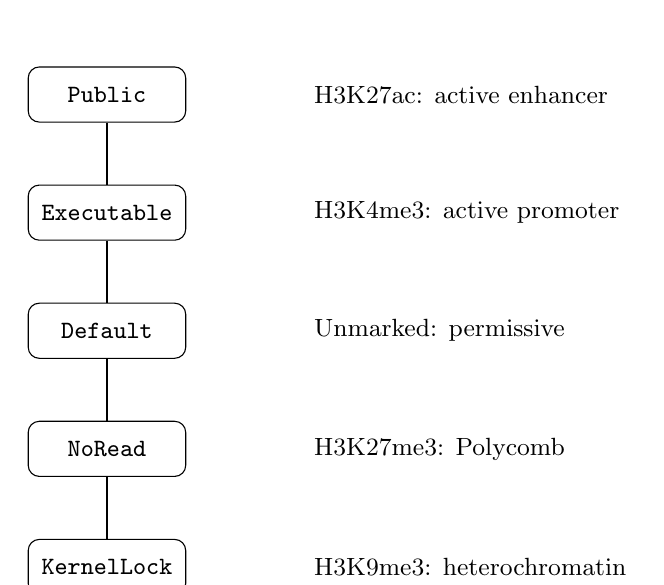
\begin{tikzpicture}[
    node distance=1.8cm,
    every node/.style={draw, rounded corners, minimum width=2cm, minimum height=0.7cm, align=center, font=\small\ttfamily}
]
    \node (pub) at (0,6) {Public};
    \node (exec) at (0,4.5) {Executable};
    \node (def) at (0,3) {Default};
    \node (noread) at (0,1.5) {NoRead};
    \node (kern) at (0,0) {KernelLock};

    \draw[-] (pub) -- (exec);
    \draw[-] (exec) -- (def);
    \draw[-] (def) -- (noread);
    \draw[-] (noread) -- (kern);

    \node[draw=none, right=1.5cm of pub, font=\small\rmfamily] {H3K27ac: active enhancer};
    \node[draw=none, right=1.5cm of exec, font=\small\rmfamily] {H3K4me3: active promoter};
    \node[draw=none, right=1.5cm of def, font=\small\rmfamily] {Unmarked: permissive};
    \node[draw=none, right=1.5cm of noread, font=\small\rmfamily] {H3K27me3: Polycomb};
    \node[draw=none, right=1.5cm of kern, font=\small\rmfamily] {H3K9me3: heterochromatin};
\end{tikzpicture}
\caption{Hasse diagram of the permission lattice $\mathcal{P}$.}
\label{fig:hasse}
\end{figure}

\section{Accessibility Lattice Product Structure}
\label{app:product}

The full accessibility lattice $\mathcal{A} = \mathbb{B} \times \mathcal{P} \times \mathcal{N}$ has $2 \times 5 \times 3 = 30$ elements. The partial order is the product order: $(b_1, p_1, n_1) \sqsubseteq (b_2, p_2, n_2)$ iff $b_1 \leq b_2$ and $p_1 \leq p_2$ and $n_1 \leq n_2$, where $\Meth < \Unmeth$, $\mathcal{P}$ is ordered as in \Cref{app:hasse}, and $\texttt{Positioned} < \texttt{Remodeled} < \texttt{Free}$.

\begin{table}[H]
\centering
\caption{Selected elements of the accessibility lattice with biological interpretation}
\label{tab:acc-elements}
\begin{tabular}{lllp{5cm}}
\toprule
\textbf{Element} & \textbf{Coordinates} & \textbf{Score} & \textbf{Biological State} \\
\midrule
$\bot$ & (M, KL, P) & 0.000 & Constitutive heterochromatin \\
PcG-silent & (U, NR, P) & 0.002 & Polycomb-silenced gene \\
Default & (U, Def, P) & 0.030 & Poised, low expression \\
Bivalent & (U, Exec$\sqcap$NR, P) & 0.002 & Stem cell bivalent \\
Active promoter & (U, Exec, R) & 0.400 & Moderately active \\
$\top$ & (U, Pub, F) & 1.000 & Maximally active \\
\bottomrule
\end{tabular}
\end{table}

\section{Categorical Diagrams}
\label{app:cat-diagrams}

\begin{figure}[H]
\centering
\begin{tikzcd}[column sep=huge, row sep=huge]
    \cat{Locus} \arrow[r, "M"] \arrow[d, "E"'] \arrow[dr, phantom, "\Downarrow\varepsilon"] & \cat{Locus} \arrow[d, "E"] \\
    \cat{Expr} \arrow[r, "\id"'] & \cat{Expr}
\end{tikzcd}
\caption{The expression functor $E$ and methylation endofunctor $M$ with the TET counit $\varepsilon$. The diagram commutes: $E \circ \varepsilon = E$ (demethylation restores the expression potential).}
\label{fig:E-M-commute}
\end{figure}

\begin{figure}[H]
\centering
\begin{tikzcd}[column sep=large, row sep=large]
    M^3 \arrow[r, "M\mu_M"] \arrow[d, "\mu_M M"'] & M^2 \arrow[d, "\mu_M"] \\
    M^2 \arrow[r, "\mu_M"'] & M
\end{tikzcd}
\quad
\begin{tikzcd}[column sep=large, row sep=large]
    M \arrow[r, "M\eta"] \arrow[dr, "\id"'] & M^2 \arrow[d, "\mu_M"] & M \arrow[l, "\eta M"'] \arrow[dl, "\id"] \\
    {} & M & {}
\end{tikzcd}
\caption{Monad coherence diagrams for the methylation monad $(M, \eta, \mu_M)$. Left: associativity. Right: unit laws.}
\label{fig:monad-coherence}
\end{figure}

\section{Enzyme-Permission Correspondence Table}
\label{app:enzyme-table}

\begin{table}[H]
\centering
\caption{Complete enzyme-permission correspondence}
\label{tab:enzyme-perm}
\begin{tabular}{llll}
\toprule
\textbf{Enzyme} & \textbf{Class} & \textbf{Mark} & \textbf{Permission Transition} \\
\midrule
DNMT3A/B & Writer & 5mC & $\Unmeth \to \Meth$ \\
DNMT1 & Writer & 5mC & $\Unmeth_{\mathrm{hemi}} \to \Meth$ \\
TET1/2/3 & Eraser & 5mC & $\Meth \to \Unmeth$ \\
EZH2 (PRC2) & Writer & H3K27me3 & Default $\to$ NoRead \\
KDM6A/UTX & Eraser & H3K27me3 & NoRead $\to$ Default \\
SUV39H1/2 & Writer & H3K9me3 & Default $\to$ KernelLock \\
KDM4A-D & Eraser & H3K9me3 & KernelLock $\to$ Default \\
SET1A/MLL & Writer & H3K4me3 & Default $\to$ Executable \\
KDM5A-D & Eraser & H3K4me3 & Executable $\to$ Default \\
p300/CBP & Writer & H3K27ac & Default $\to$ Public \\
HDAC1-11 & Eraser & H3K27ac & Public $\to$ Default \\
HP1$\alpha/\beta$ & Reader & H3K9me3 & KernelLock $\to$ KernelLock \\
BRD4 & Reader & H3K27ac & Public $\to$ Public \\
MBD1-4 & Reader & 5mC & $\Meth \to \Meth$ \\
\bottomrule
\end{tabular}
\end{table}

\end{document}
